%
\documentclass{tstextbook}

\usepackage{mathematica}
\usepackage[T1]{fontenc}
\usepackage[scaled=0.9]{DejaVuSansMono}
\usepackage[export]{adjustbox}

\usepackage{amssymb}
\usepackage{amsmath}
\usepackage{graphicx}

\begin{document}

\tsbook{Probabilistic Modeling\\ with the\\ Wolfram Language}
       {Gerhard Hejc}
       {Cover Designer}
       {2020}
       {xxxxx}{xxx--xx--xxxx--xx--x}{0.0}
       {Publisher}
       {City}

%---------------------------------------------------------------------------
% Chapters
%---------------------------------------------------------------------------
%---------------------------------------------------------------------------
\chapter*{Preface}

The book originally developed from talks and lecture notes given at the Fraunhofer institute in Nuremberg, Germany as an introduction to probabilistic modeling. The goal was primarily to provide the students with a minimal set of mathematical tools and concepts to do probabilistic computations by themselves and to apply it to real-world problems. This sounds easier than it actually is, because even conceptually easy problems can lead to results, which contradicts intuition like the famous Monty Hall problem.\\

There are basically two main branches of probabilistic modeling: simulation and inference. The first uses a probabilistic model based on a theory to make predictions or simulate the outcome of an experiment or a measurement, while the second one uses collected data to create a probabilistic model. The term probabilistic means the ability to include uncertainty into the model. Uncertainty in the first case is entering through only imprecisely known parameters,  hidden variables and approximations, while in the second case it depends on the degree of knowledge about the noise which is inherently present in the data or the process how the data was generated or how many parameters are necessary to describe the data. Including uncertainty is not an option, but a necessity to make precise statements about the reliability of our results.  \\    

A lot of exciting developments took place in this field in the last years. Most of the non-trivial calculations are almost impossible to be done without a computer, so the question quickly arises what is the appropriate software tool for doing this kind of calculations. Because of the availability of a large number of good software, it is merely somebody's preference towards one or the other, but in this book the Wolfram language is chosen for several reasons.\\

The Wolfram language \cite{wolfram2015, don2018} has a clear and consistent design with a syntax close to the mathematical notation and has all the built-in knowledge to perform symbolic calculations where results in a closed-form are available and numerical evaluations in the case where this is not possible. Especially the Probability and Statistics part, which is used heavily in this book, has been improved significantly in the newer version of the language and the available functions can be easily applied to all kind of statistical problems. The visualization capabilities of the Wolfram language are outstanding and every figure in this book was generated with the version integrated into Mathematica 12.0 \cite{mathematica12}.\\

This is not the first book about this topic, but builds on the work of others. There are many great books available, and these recommendations are definitely not exhaustive, but only a subjective subset:

\begin{itemize}
\item 
David Barber's book \textbf{Bayesian Reasoning and Machine Learning} \cite{barber2011} is one of the best books, which covers extensively all topics in great detail and clarity.
\item
Bendat and Piersol's \textbf{Random Data: Analysis and Measurement Procedures} \cite{bendat2010} is a classic book published first 1971, but still a clear and well-written reference about the analysis of random data, especially time series data.
\item
Simon Sirca's book \textbf{Probability for Physicists} \cite{sirca2016} is a good introduction with many examples from physics.
\item
Glen Cowan's book \textbf{Statistical Data Analysis} \cite{cowan1998} is a concise and well-written treatise targeting mainly readers of the particle physics community.   
\end{itemize}

Some knowledge in Linear Algebra and Calculus is also required e.g. see Murray Spiegel's book \textbf{Schaum's Outline of Advanced Mathematics for Engineers and Scientists} \cite{spiegel2009} for an excellent coverage of all the mathematical methods and tools used by engineers and scientists. There is also another book by the same author completely dedicated to probability and statistics \cite{spiegel2012}, which consists of 897 fully solved problems and 20 online videos.\\

A great tool for exploring univariate probability distributions built into the Wolfram Language is the \textbf{The Ultimate Univariate Probability Distribution Explorer}, which can be downloaded from \cite{marichev2013}.\\

There is already a very good book \textbf{Introduction to Probability with Mathematica} by Kevin J. Hastings \cite{hastings2001} with a similar intention than this one. The second edition is based on Mathematica 7.0 and it is highly recommended as a complementary reading.\\

Nevertheless the goal of this book is a bit different. We want to cover only the relevant topics and concepts, which are necessary for building and analyzing probabilistic models and applying them to all kind of problems. Therefore it does not claim to be a complete treatise of the subject, but a rather concise introduction to bring the reader as fast as possible into a state to perform computations and to understand its results.    

%---------------------------------------------------------------------------
\chapter{Basic Concepts}

\begin{summary}
  This first chapter introduces the basic concepts. The starting point in other text books about this topic is typically the definition of probability based on the Kolmogorov axioms. This book chooses a different approach and puts the main focus on the probability density. Everything else including probability is derived from this quantity. The reason for this choice is mainly that the result of almost every non-trivial probabilistic calculation in physics or mathematics is always a (conditional) probability density. It includes the complete information about a random process and plays a central role in the description of probabilistic systems. As we will see, it contains also deterministic systems as a special case and is therefore a generalization of a function for the case, when uncertainty comes into play.     
\end{summary}

%---------------------------------------------------------------------------
\section{Probability Density}

The probability density is a generalized function, which describes the distribution of values of an random variable. Generalized means here that it can contain Dirac delta functions. It describes the outcome of an experiment or measurement, where the value of the random variable is determined. The exact value of an outcome is unpredictable, but the frequency of the occurrence of a value is described by the probability density. Even if the probability density is typically a function, the value at a specific point has no direct meaning, only the integral over a certain range of values can be interpreted as probability. The terms probability density function (pdf) or probability distribution or simply distribution are used synonymously for a probability density. So when we write $p(x)$, it means the probability density associated with the random variable $x$ or $x$ is distributed as $p(x)$. In the function $p(x)$ $x$ is only a placeholder and can be replaced by another symbol e.g. $u$. In this case we write $p(x=u)$, which means that in the functional form of the pdf associated with the random variable $x$, we use $u$ as an argument. This notation is also used when we set the random variable to a fixed value e.g. $p(x=x_0)$. Any dependence of the probability density on a set of parameters $\theta_1,\theta_2,\ldots,\theta_n$ will be written as 
$p(x\,\vert\,\theta_1,\theta_2,\ldots,\theta_n)$ or in short form $p(x\,\vert\,\boldsymbol{\theta})$.\\  

The definition of a probability density is given below:

\begin{definition}[Probability Density]
  \label{th:probabilitydensity}
  \index{probability density}
  A probability density $p(x)$ is a generalized non-negative function of a variable
  $x$ with a support of $[-\infty,+\infty]$ such that
  \begin{equation}
    \int_{-\infty}^{+\infty}p(x)dx=1
  \end{equation}
\end{definition}
The dimension of a probability density $p(x)$ is the inverse of the dimension of the associated random variable $x$.\\

A random variable is defined as
\begin{definition}[Random Variable]
  \label{th:randomvariable}
  \index{random variable}
  A real-valued continuous variable $x$ is called a random variable if $x$ is distributed as $p(x)$ (also written as $x\sim p(x)$). This means that the distribution of values of the random variable $x$ is completely described by the probability density $p(x)$.
\end{definition}

A random variable with a finite support $[a,b]$ can be described by a probability density, which is zero outside of the interval $[a,b]$.\\

A probability density of two or more random variables is called a joint probability density e.g. $p(x,y)$ in the case of two random variables $x$ and $y$. The normalization condition is given by 
  \begin{equation}
    \int_{-\infty}^{+\infty}\int_{-\infty}^{+\infty}p(x,y)dxdy=1
  \end{equation}
Integrating only over one random variable e.g. $y$, the result is again a valid probability density $p(x)$. This operation is called marginalization. Therefore the simplest way to construct a joint (or multi-variate) probability density out of uni-variate probability densities is by multiplication e.g. $p(x,y)=p(x)p(y)$.

\begin{remark}
\textit{One word of caution: if we say that $x$ is distributed as $p(x)$ and $y$ is distributed as $p(y)$, that does not mean that the probability distributions have the same functional form, but it is kept open if they are identical or different. Whenever they are identical, we explicitly mention this and say that $x$ and $y$ are identically distributed.}
\end{remark}

For multi-variate probability densities we follow the notation of writing the argument in bold letters or with an index range subscript e.g. $p(\mathbf{x})$ or $p(x_{1:n})$ is the short form for the joint probability density $p(x_1,x_2,\ldots,x_n)$. \\

The Wolfram Language represents a probability density by the function \texttt{ProbabilityDistribution} e.g. the following code creates a pdf $\frac{\sqrt{2}}{\pi\alpha\left(1+\left(\frac{x}{\alpha}\right)^4\right)}$

\begin{mathematica}
dist = ProbabilityDistribution[Sqrt[2]/(Pi*\[Alpha])/(1 + (x/\[Alpha])^4),
                               {x, -Infinity, Infinity}, 
                               Assumptions -> {\[Alpha] > 0}];
\end{mathematica} 
The \texttt{Assumptions} option $\alpha > 0$ is necessary to guarantee the non-negativity of the pdf. The function, which is provided as the first argument, must be normalized to unity or if not, the option \texttt{ Method -> "Normalize"} must be explictely set. An equivalent definition would be
\begin{mathematica}
dist = ProbabilityDistribution[1/(1 + (x/\[Alpha])^4),
                               {x, -Infinity, Infinity},
                               Method -> "Normalize",
                               Assumptions -> {\[Alpha] > 0];
\end{mathematica} 
The distribution instance can then be used for plotting.
\begin{mathematica}
Plot[{PDF[dist, x] //. {\[Alpha] -> 1},
      PDF[dist, x] //. {\[Alpha] -> 2}},
      {x, -4, 4}, Filling -> Axis,
      PlotLegends -> Placed[{"\[Alpha]=1", "\[Alpha]=2"}, Right]]
\end{mathematica}

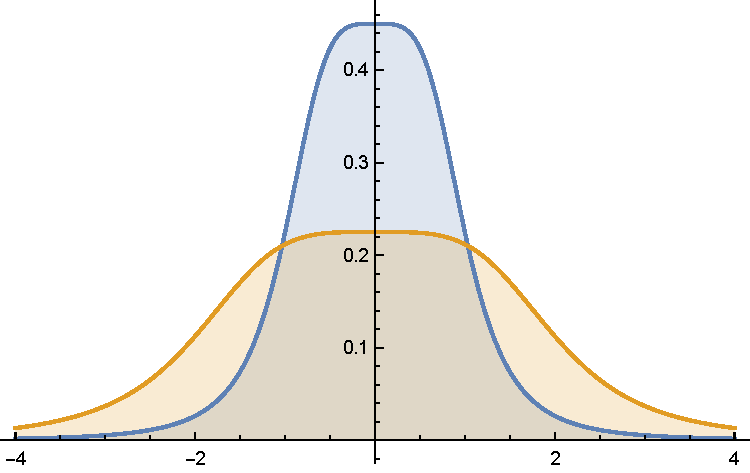
\includegraphics[scale=0.7, center]{images/probability_distribution.pdf}

\texttt{ProbabilityDistribution} can be also used for the creation of joint probability densities. 
\begin{mathematica}
dist = ProbabilityDistribution[
          Gamma[3/4]/(Gamma[5/4]*Sqrt[2 Pi^3])/(1 + x^4 + y^4),
          {x, -Infinity, Infinity},
          {y, -Infinity, Infinity}];
Plot3D[PDF[dist, {x, y}], {x, -4, 4}, {y, -4, 4}, 
       PlotRange -> {0, 0.2}, PlotPoints -> {50, 50}]
\end{mathematica}

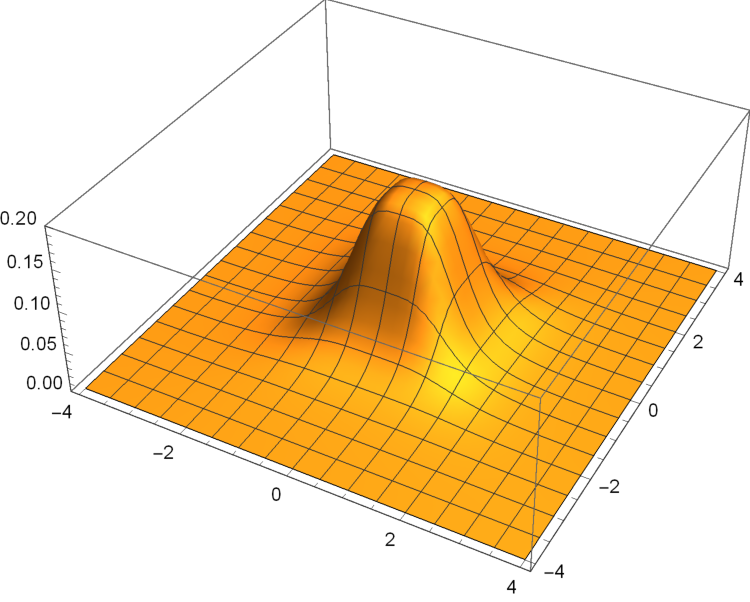
\includegraphics[scale=0.7, center]{images/joint_probability_distribution.pdf}

\begin{example}[The Univariate Normal Distribution]
  The most important probability density is the Normal (or Gauss) distribution $\mathcal{N}\left(x\,\vert\,\mu,\sigma^2\right)$, which has the functional form
  \begin{equation}
    \frac{1}{\sqrt{2\pi\sigma^2}}\exp{-\frac{(x-\mu)^2}{2\sigma^2}}
  \end{equation}
  The function has two free parameters $\mu$ (mean) and $\sigma$ (standard deviation) and fulfills the normalization condition for any value of $\mu$ and $\sigma$.
    \begin{equation}
    \frac{1}{\sqrt{2\pi\sigma^2}}\int_{-\infty}^{+\infty}\exp{-\frac{(x-\mu)^2}{2\sigma^2}}dx=
    \frac{1}{\sqrt{2\pi}}\int_{-\infty}^{+\infty}\exp{-\frac{x^2}{2}}dx=1
  \end{equation}
  where the variable transformation $x\rightarrow\frac{x-\mu}{\sigma}$ was used.\\

The notation $\mathcal{N}\left(x\,\vert\,\mu,\sigma^2\right)$ instead of $\mathcal{N}\left(x\,\vert\,\mu,\sigma\right)$ is motivated by the fact that the functional form only depends on $\sigma^2$ and by the generalization to the multi-variate Normal distribution, which is discussed in the next example.\\

The Wolfram Language implements the Normal distribution as \texttt{NormalDistribution}. Note that the second argument to \texttt{NormalDistribution} is the standard deviation $\sigma$, not the variance $\sigma^2$.
\begin{mathematica}
Plot[Table[PDF[NormalDistribution[0, \[Sigma]], x],
           {\[Sigma], {.75, 1, 2}}] // Evaluate,
     {x, -6, 6}, Filling -> Axis, 
     PlotLegends -> Placed[{"\[Sigma]=0.75","\[Sigma]=1","\[Sigma]=2"}, Right]]
\end{mathematica}

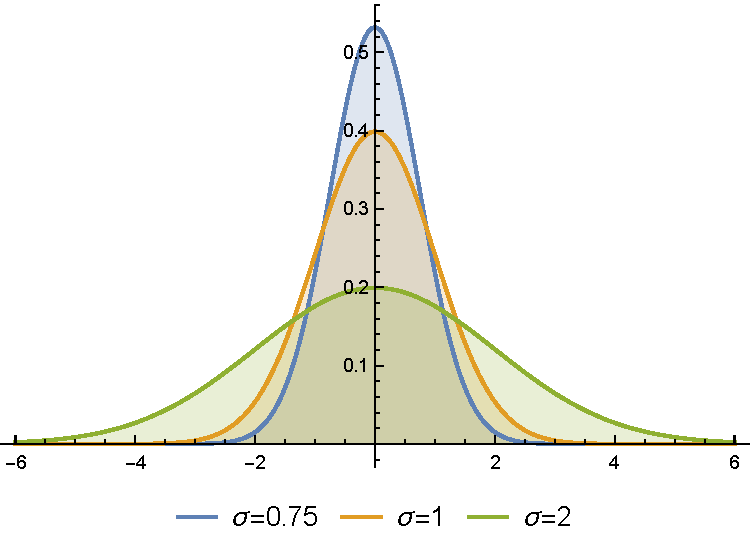
\includegraphics[scale=0.8, center]{images/normal_distribution.pdf}
\end{example}

\begin{example}[The Multivariate Normal Distribution]
  The multi-variate Normal (or Gauss) distribution
  $\mathcal{N}\left(\mathbf{x}\,\vert\,\boldsymbol{\mu},\boldsymbol{\Sigma}\right)$ has the functional form
  \begin{equation}
    \frac{1}{\sqrt{2\pi \det(\boldsymbol{\Sigma})}}\exp{-\frac{1}{2}(\mathbf{x}-\boldsymbol{\mu})^T\boldsymbol{\Sigma}^{-1}(\mathbf{x}-\boldsymbol{\mu})}
  \end{equation}
with $\mathbf{x}=x_{1:n}$,$\boldsymbol{\mu}=\mu_{1:n}$ and $\boldsymbol{\Sigma}=\Sigma_{1:n,1:n}$. $\boldsymbol{\Sigma}$ is called the covariance matrix and is symmetric $\boldsymbol{\Sigma}^T=\boldsymbol{\Sigma}$, so it has only $\frac{n(n+1)}{2}$ independent parameters. Therefore the multi-variate Normal distribution has $\frac{n(n+3)}{2}$ parameters.\\

The corresponding function in the Wolfram Language is \texttt{MultinormalDistribution}. \begin{mathematica}
Plot3D[PDF[MultinormalDistribution[{0, 0}, {{2, 1}, {1, 2}}], {x, y}],
       {x, -4, 4}, {y, -4, 4}, PlotPoints -> {50, 50}]
\end{mathematica}
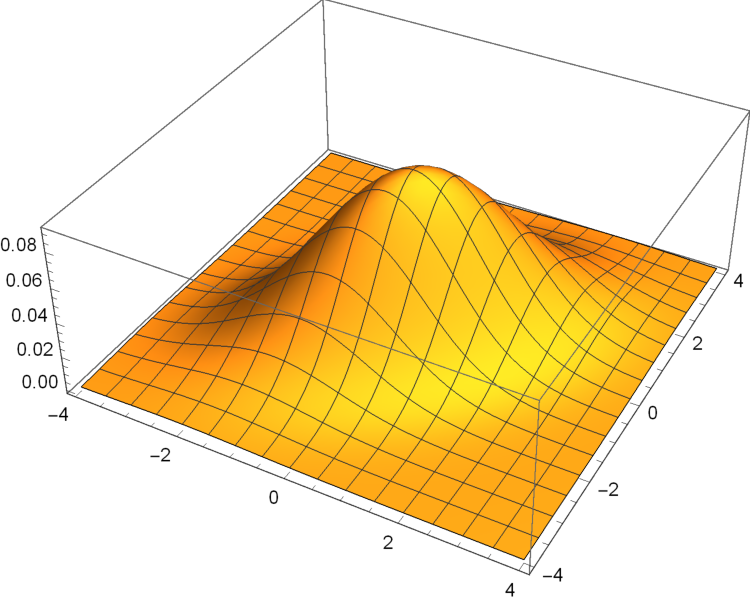
\includegraphics[scale=0.8, center]{images/multi_normal_distribution.pdf}

The function \texttt{MarginalDistribution} can be used to reduce the number of variables in a multi-variate distribution. The result of
\begin{mathematica}
MarginalDistribution[MultinormalDistribution[{0, 0}, {{2, 1}, {1, 2}}], 1]
\end{mathematica}
is the uni-variate Normal distribution $\mathcal{N}\left(x\,\vert\,\mu=0,\sigma^2=2\right)$. The second argument can be a single index or a list of multiple indices of the variables, which should be present in the new distribution.   
\end{example}

\begin{theorem}[Multivariate Normal Distribution under Affine Transformation]
  \label{th:multivariatenormaldistributionunderaffinetransformation}
  \index{linear transformation}
An important property of the multi-variate Normal distribution is that the result of an affine transformation $\mathbf{x}'=\mathrm{M}\mathbf{x}+\mathbf{b}$ with a $n\times n$ matrix $\mathrm{M}$ and a $n\times 1$ vector $\mathbf{b}$ is again a multi-variate Normal distribution   
  \begin{equation}
  \mathcal{N}\left(\mathbf{x}\,\vert\,\boldsymbol{\mu},\boldsymbol{\Sigma}\right)=
  \vert\det(M)\vert\,\mathcal{N}\left(\mathbf{x}'\,\vert\,\mathrm{M}\boldsymbol{\mu}+\mathbf{b},\mathrm{M}\boldsymbol{\Sigma}\mathrm{M}^T\right)
  \end{equation}
\end{theorem}
\begin{proof}
  \begin{equation}
\mathcal{N}\left(\mathbf{x}'\,\vert\,\mathrm{M}\boldsymbol{\mu}+\mathbf{b},\mathrm{M}\boldsymbol{\Sigma}\mathrm{M}^T\right)=
 \frac{1}{\sqrt{2\pi \det\left(\mathrm{M}\boldsymbol{\Sigma}\mathrm{M}^T\right)}}\exp{-\frac{1}{2}(\mathbf{x}-\boldsymbol{\mu})^T\mathrm{M}^T\left(\mathrm{M}\boldsymbol{\Sigma}\mathrm{M}^T\right)^{-1}\mathrm{M}(\mathbf{x}-\boldsymbol{\mu})}
 \end{equation}
 Using $\det\left(\mathrm{M}\boldsymbol{\Sigma}\mathrm{M}^T\right)=\det(\mathrm{M})^2 \det(\boldsymbol{\Sigma})$ and $\mathrm{M}^T\left(\mathrm{M}\boldsymbol{\Sigma}\mathrm{M}^T\right)^{-1}\mathrm{M} = \mathrm{M}^T(\mathrm{M}^T)^{-1}\boldsymbol{\Sigma}^{-1}\mathrm{M}^{-1}\mathrm{M}=\boldsymbol{\Sigma}^{-1}$, the right hand side of the expression simplifies to
  \begin{equation}
\mathcal{N}\left(\mathbf{x}'\,\vert\,\mathrm{M}\boldsymbol{\mu}+\mathbf{b},\mathrm{M}\boldsymbol{\Sigma}\mathrm{M}^T\right)=
 \frac{1}{\vert\det(M)\vert\sqrt{2\pi \det\left(\boldsymbol{\Sigma}\right)}}\exp{-\frac{1}{2}(\mathbf{x}-\boldsymbol{\mu})^T\boldsymbol{\Sigma}^{-1}(\mathbf{x}-\boldsymbol{\mu})}
 \end{equation}
 The normalization condition is also fulfilled.
   \begin{equation}
\int_{-\infty}^{+\infty}d\mathbf{x}'\mathcal{N}\left(\mathbf{x}'\,\vert\,\mathrm{M}\boldsymbol{\mu}+\mathbf{b},\mathrm{M}\boldsymbol{\Sigma}\mathrm{M}^T\right)=
 \frac{\vert\det(M)\vert}{\vert\det(M)\vert}\int_{-\infty}^{+\infty}d\mathbf{x}\mathcal{N}\left(\mathbf{x}\,\vert\,\boldsymbol{\mu},\boldsymbol{\Sigma}\right)=1
 \end{equation}
 The short-hand notation $\int_{-\infty}^{+\infty}d\mathbf{x}$ is used for the $n$-dimensional integral $\prod_{i=1}^n\int_{-\infty}^{+\infty}dx_i$.
 \end{proof}

\begin{example}[The Uniform Distribution]
  The simplest probability density is the uniform distribution $\mathcal{U}(x\,\vert\,\alpha,\beta)$, which has the functional form
  \begin{equation}
    \frac{1}{\beta-\alpha}\Theta(\beta-x)\Theta(x-\alpha)
  \end{equation}
  with $\beta>\alpha$. $\Theta(x)$ is the Heaviside step function, which is defined as
    \begin{equation}
    \Theta(x)=\begin{cases}0 & x < 0 \\
1 & x\geqq 0 \\
\end{cases}
  \end{equation}
  The two $\Theta$-functions guarantee that the probability density is zero outside the interval $[a,b]$. The normalization condition can be easily verified by
  \begin{equation}
    \frac{1}{\beta-\alpha}\int_{-\infty}^{+\infty}\Theta(\beta-x)\Theta(x-\alpha)dx
    =\frac{1}{\beta-\alpha}\int_{\alpha}^{\beta}dx=\frac{\beta-\alpha}{\beta-\alpha}=1
  \end{equation}
  
Wolfram Language has a function \texttt{UniformDistribution} with a list argument $\{\alpha,\beta\}$.

\begin{mathematica}
Plot[Table[PDF[UniformDistribution[{0, \[Beta]}], x], 
           {\[Beta], {1, 2, 4}}] // Evaluate, 
     {x, -1, 5}, Filling -> Axis, PlotRange -> {0, 1},
     PlotLegends -> Placed[{"\[Beta]=1", "\[Beta]=2", "\[Beta]=4"}, Right]]
\end{mathematica}
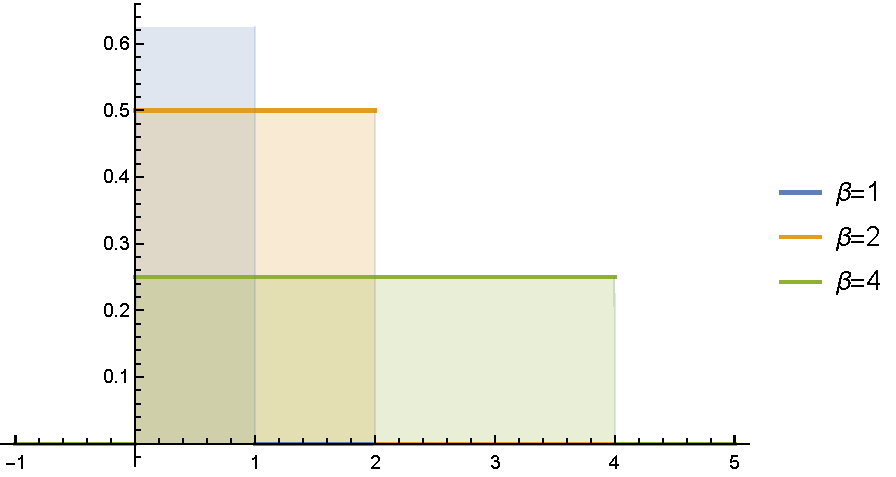
\includegraphics[scale=1, center]{images/uniform_distribution.pdf}  
\end{example}

\begin{exercise}
Show that the sum of two random variables distributed as $\mathcal{U}(x\,\vert\,\alpha,\beta)$ is given by a triangular distribution between the two end points $2\alpha$ and $2\beta$ and a peak at $\alpha+\beta$, which is built into the Wolfram Language as \texttt{TriangularDistribution}.
\end{exercise}

%---------------------------------------------------------------------------
\section{Probability}

Probability is defined in terms of the probability density in the following way.

\begin{definition}[Probability]
  \label{th:probability}
  \index{probability}
  The probability of $x$ taking a value between $x_1$ and $x_2$ is given by
  \begin{equation}
    P(x_1\leqq x\leqq x_2)=\int_{x_1}^{x_2}p(x)dx
  \end{equation}
  In the case of a joint probability density, the probability of $x$ taking a value between $x_1$ and $x_2$ and $y$ taking a value between $y_1$ and $y_2$ is given by
  \begin{equation}
    P(x_1\leqq x\leqq x_2\:\ \& \:y_1\leqq y\leqq y_2)=\int_{x_1}^{x_2}\int_{y_1}^{y_2}p(x,y)dxdy
  \end{equation}
  The generalization to the case of a multi-variate probability density with more than 2 random variables is self-explanatory. 
\end{definition}
The convention to write probabilities with an upper case $P$ and probability densities with a lower case $p$ is adapted throughout the book.

We will now show that all the properties of a probability (also known as Kolmogorov axioms) follow from this definition.

\begin{theorem}[Probability Axioms]
  \label{th:probabilityaxioms}
  \index{probability axioms}
  The probability satisfies the following 3 axioms: 
  \begin{enumerate}
\item 
The probability is a non-negative real number.
\item
The probability of $x$ taking a value between $[-\infty,+\infty]$ is 1.
\item
A set of disjoint intervals $\mathcal{I}_i$ with $i=1,\ldots,n$ has the probability $\sum_{i=1}^n P(\mathcal{I}_i)$.
\end{enumerate}
\end{theorem}
\begin{proof}
Based on the definition of the probability as integral over a probability density, the proof is rather trivial. The first axiom follows directly from the non-negativity of the probability density, the second axiom from the normalization condition and the third axiom from the additivity of integrals over disjoint integration intervals, which simply follows from the interpretation of an integral as an area under a curve.
\end{proof}
Because probability is related to the integral of a probability density, a cumulative distribution function is defined as
\begin{definition}[Cumulative Distribution Function]
  \label{th:cumulativedistributionfunction}
  \index{cumulative distribution function}
  A cumulative distribution function (cdf) of a random variable $x$ is given by
  \begin{equation}
    \Phi(x)=\int_{-\infty}^{x}p(x=x')dx'
  \end{equation}
The probability of $x$ taking a value between $x_1$ and $x_2$ can then be written as the difference of two cumulative distribution functions evaluated at $x_2$ and $x_1$.
  \begin{equation}
    P(x_1\leqq x\leqq x_2)=\Phi(x_2)-\Phi(x_1)
  \end{equation} 
\end{definition}

Wolfram Language has built in the functions \texttt{Probability} and \texttt{CDF}, which can be applied to any distribution e.g.
\begin{mathematica}
Probability[x <= 0, x \[Distributed] NormalDistribution[]]
\end{mathematica}
with the result $\frac{1}{2}$, which can be also obtained using
\begin{mathematica}
CDF[NormalDistribution[], 0]
\end{mathematica}
The cumulative distribution function of the Normal and the Uniform distribution is shown in the next figures
\begin{mathematica}
Plot[Table[CDF[NormalDistribution[0, \[Sigma]], x],
     {\[Sigma], {0.5, 1, 2}}] // Evaluate,
     {x, -4, 4}, AxesLabel -> {"x", "\[CapitalPhi](x)"}, 
     Filling -> Axis, PlotLegends -> 
     Placed[{"\[Sigma]=0.5", "\[Sigma]=1", "\[Sigma]=2"}, Right]]
\end{mathematica}

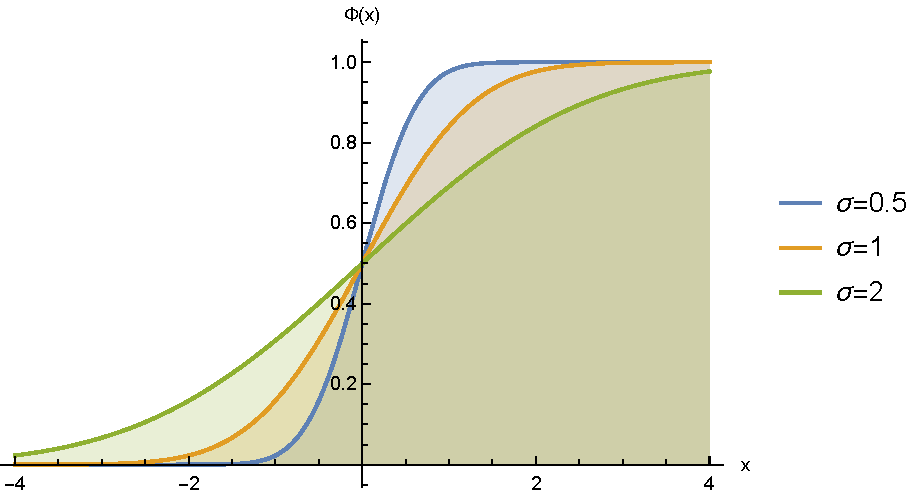
\includegraphics[scale=0.8, center]{images/cumulative_normal_distribution.pdf}

\begin{mathematica}
Plot[Table[CDF[UniformDistribution[{0, \[Beta]}], x],
     {\[Beta], {1, 2, 3}}] // Evaluate,
     {x, -1, 4}, AxesLabel -> {"x", "\[CapitalPhi](x)"}, 
     Filling -> Axis, PlotLegends -> 
  Placed[{"\[Beta]=1", "\[Beta]=2", "\[Beta]=3"}, Right]]
\end{mathematica}

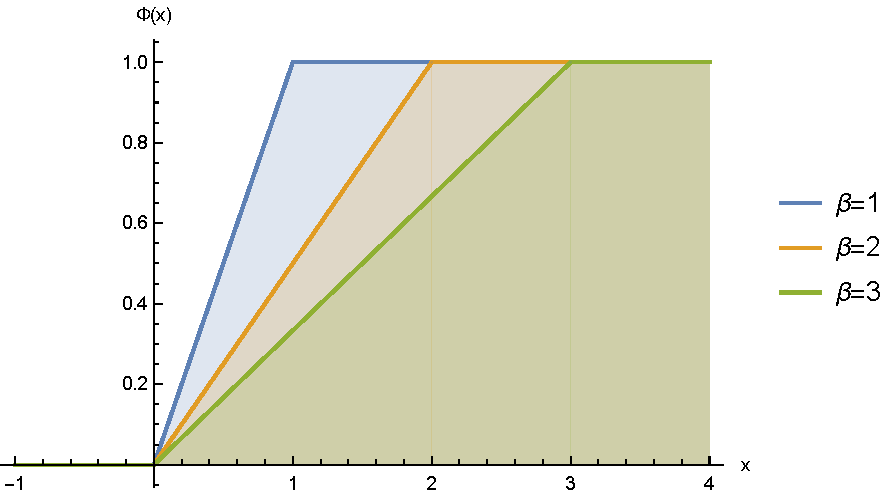
\includegraphics[scale=0.8, center]{images/cumulative_uniform_distribution.pdf}

%---------------------------------------------------------------------------
\section{Conditional Probability Density}

Almost all probability densities are conditional probability densities, because they depend on various parameters and/or other random variables. We will treat parameters and random variables behind the condition symbol in the same way, which means that we assume that they have a fixed value, when the probability density is evaluated. The only difference is that a random variable can be in front of or behind the condition symbol, whereas parameters can only be placed behind it.

A conditional probability density $p(x\,\vert\, y,\theta)$ means a probability density of $x$ given $y$ (a random variable) and $\theta$ (a parameter).

\begin{definition}[Conditional Probability Density]
  \label{th:conditionalprobabilitydensity}
  \index{conditional probability density}
  The conditional probability $p(x\,\vert\, y,\theta)$ is defined by
  \begin{equation}
    p(x\,\vert\, y,\theta)=\frac{p(x, y\,\vert\, \theta)}{p(y\,\vert\, \theta)}=\frac{p(x, y\,\vert\, \theta)}{\int_{-\infty}^{+\infty}p(x,y\,\vert\, \theta)dx}
  \end{equation}
  A similar equation holds for $p(y\,\vert\, x,\theta)$
  \begin{equation}
    p(y\,\vert\, x,\theta)=\frac{p(x, y\,\vert\, \theta)}{p(x\,\vert\, \theta)}=\frac{p(x, y\,\vert\, \theta)}{\int_{-\infty}^{+\infty}p(x,y\,\vert\, \theta)dy}
  \end{equation}
  Eliminating the joint probability density $p(x, y\,\vert\, \theta)$ leads to the Bayes rule
  \begin{equation}
    p(x\,\vert\, y,\theta)=\frac{p(y\,\vert\, x,\theta)p(x\,\vert\, \theta)}{p(y\,\vert\, \theta)}
  \end{equation} 
\end{definition}

A joint probability density $p(\mathbf{x}\,\vert\, \mathbf{y},\boldsymbol{\theta})$ can be decomposed into univariate conditional probability densities by iteratively applying Bayes rule.
  \begin{equation}
  \label{eq:decomposition}
    p(\mathbf{x}\,\vert\, \mathbf{y},\boldsymbol{\theta})=p(x_{1:n}\,\vert\, \mathbf{y},\boldsymbol{\theta})=p(x_1\,\vert\, x_{2:n},\mathbf{y},\boldsymbol{\theta})
\underbrace{p(x_{2}\,\vert\, x_{3:n},\mathbf{y},\boldsymbol{\theta})\overbrace{\ldots p(x_{n-1}\,\vert\, x_n,\mathbf{y},\boldsymbol{\theta})
p(x_{n}\,\vert\, \mathbf{y},\boldsymbol{\theta})}^{p(x_{3:n}\,\vert\, \mathbf{y},\boldsymbol{\theta})}
}_{p(x_{2:n}\,\vert\, \mathbf{y},\boldsymbol{\theta})}
  \end{equation}
This decomposition is not unique. Any permutations of $\mathbf{x}$ is possible here.\\

\textit{The question is: what is the best choice for this decomposition?}\\

There is no general answer here, but if you are able to exploit the conditional independence of random variables as often as possible by using
  \begin{equation}
    p(x\,\vert\, y,\theta)=p(x\,\vert\, \theta)
  \end{equation}
then the individual terms in the product will simplify significantly.
The statement $x$ is conditionally independent from $y$ means that the functional form of the probability density of $x$ is the same regardless of the value of $y$.\\

\begin{remark}
Expressions with a product of probability densities will occur very often and are subject to numerical underflow. It is therefore recommended to perform numerical evaluations always with the logarithm of a probability density. It does not matter if it is the natural logarithm (we use $\ln$ or $\log$ interchangeably) or the logarithm with base 2 or 10 (in this case we write explicitely $\log_2$ or $\log_{10})$. The crucial point is that a product of pdf's is converted into a sum of logarithms of pdf's.
\end{remark}

\begin{example}[A Normal Distribution with an Uncertain Parameter]
Let's assume that a random variable $x$ is distributed as $\mathcal{N}\left(x\,\vert\,\mu,\sigma^2\right)$, but we are uncertain about its mean $\mu$. We can only say that its value is between $\alpha$ and $\beta$. So this uncertainty turns the parameter $\mu$ into a random variable distributed as $\mathcal{U}\left(\mu\,\vert\,\alpha,\beta\right)$ and we can ask what is the joint probability density $p(x,\mu)$. 
  \begin{equation}
  p\left(x,\mu\,\vert\,\sigma^2,\alpha,\beta\right)=\mathcal{N}\left(x\,\vert\,\mu,\sigma^2\right)\mathcal{U}\left(\mu\,\vert\,\alpha,\beta\right)
  \end{equation}
Even if $\mu$ is now an random variable, the functional form of $\mathcal{N}\left(x\,\vert\,\mu,\sigma^2\right)$ is the same as before. This is the reason why no distinction is made between parameters and random variables behind the condition bar.
\end{example}

The Wolfram Language has no special function for conditional pdf's, because basically every probability density with parameters is a conditional pdf. Nevertheless it may be necessary to go from a joint pdf $p(x,y)$ to a conditional pdf $p(x\,\vert\, y)$.
\begin{mathematica}
joint = BinormalDistribution[{\[Mu]1, \[Mu]2}, {\[Sigma]1, \[Sigma]2}, \[Rho]];
dist2 = MarginalDistribution[joint, 2];
cond = ProbabilityDistribution[
           PDF[joint, {x1, x2}]/PDF[dist2, x2],
           {x1, -Infinity, Infinity}]
\end{mathematica}
The result is
  \begin{equation}
  \label{eq:conditional_binormal_distribution}
    p\left(x_1\,\vert\, x_2, \mu_1, \mu_2, \sigma_1, \sigma_2, \rho\right)=\frac{\exp \left(\frac{(x_2-\mu_2)^2}{2 \sigma_2^2}-\frac{\frac{(x_1-\mu _1)^2}{\sigma_1^2}-\frac{2 \rho  (x_1-\mu_1) (x_2-\mu_2)}{\sigma_1 \sigma_2}+\frac{(x_2-\mu_2)^2}{\sigma_2^2}}{2 \left(1-\rho ^2\right)}\right)}{\sqrt{2 \pi } \sqrt{1-\rho ^2} \sigma_1}
  \end{equation}
The normalization condition can be checked with
\begin{mathematica}
Integrate[PDF[cond, x], {x, -Infinity, Infinity}, 
   Assumptions -> {Element[\[Sigma]1, NonNegativeReals], 
                   Element[\[Sigma]2, NonNegativeReals], 
                   Element[\[Rho], NonNegativeReals],
                   \[Rho] < 1, \[Sigma]1 > 0}]
\end{mathematica}
The result is exactly $1$ if the constraints $\rho < 1$ and $\sigma_1 > 0$ are taken into account, because eq. \ref{eq:conditional_binormal_distribution} is singular at $\rho = 1$ and $\sigma_1 = 0$. 

%---------------------------------------------------------------------------
\section{Deterministic Functions}
We will now show that every function can be written as a conditional probability density. This will allow us to treat everything as probability density and mix deterministic and random behavior in our models.

Let's study the Normal distribution in the limit $\sigma^2\rightarrow 0$, where the uncertainty of observing the value $\mu$ changes to certainty and the outcome of the random variable $x$ is always $\mu$.

\begin{example}[The Normal Distribution with zero variance]
  \begin{equation}
    \lim_{\sigma^2\rightarrow 0}\mathcal{N}\left(x\,\vert\,\mu,\sigma^2\right)= \lim_{\sigma^2\rightarrow 0}\frac{1}{\sqrt{2\pi\sigma^2}}\exp{-\frac{(x-\mu)^2}{2\sigma^2}}=
\delta\left(x-\mu\right)
  \end{equation}
\end{example}

As we can see from the example, the probability density becomes a Dirac delta function with the functional relation $x=\mu$ as argument.

\begin{definition}[Deterministic Probability Density]
  \label{th:deterministicprobabilitydensity}
  \index{deterministic probability density}
  Any function $y=f(x)$ can be written as conditional probability density in the following way.
  \begin{equation}
    p(y\,\vert\,x)=\delta\left(y-f(x)\right)
  \end{equation} 
\end{definition}

A common use-case is that we have a conditional probability density, which will be become deterministic by including hidden (or latent) random variables. The random character of a quantity could be completely originate from another random variable and as soon as this other random variable has been identified and included, the conditional probability density can be replaced by an expression of the form shown above if the functional dependency on the hidden variable is known.

Another consequence is that an integration over $y$ can be carried out immediately using
  \begin{equation}
    \int_{-\infty}^{+\infty}\delta\left(y-f(x)\right)g(y)dy = g(f(x))
  \end{equation} 

Another use-case are variable transformations from a random variable $x$ with a known probability density $p(x)$ to another variable $y=f(x)$.\\

\textit{The question is: what is the pdf of $y$?}\\

The starting point for the case with two random variables $x$ and $y$ is always the joint probability density $p(x,y)$. Because we are only interested in the pdf of $y$, we marginalize over $x$.

  \begin{equation}
    p(y)=\int_{-\infty}^{+\infty}p(x,y)dx=
    \int_{-\infty}^{+\infty}p(y\,\vert\, x)p(x)dx=\int_{-\infty}^{+\infty}\delta\left(y-f(x)\right)p(x)dx
  \end{equation}
Using the following identity for the Dirac delta function
  \begin{equation}
   \delta\left(y-f(x)\right)=\sum_{i=1}^{n}\frac{1}{\vert f'(x_i)\vert}\delta(x-x_i(y))
  \end{equation}
where $x_i(y)$ are all $n$ solutions of $y=f(x)$ and $f'(x_i)$ is the derivative of $f(x)$ with respect to $x$ evaluated at $x=x_i(y)$, one can carry out the integration over $x$ with the result
  \begin{equation}
    p(y)=\sum_{i=1}^{n}\frac{1}{\vert f'(x_i)\vert}p\left(x=x_i(y)\right)
  \end{equation}

\begin{example}[The Square of a Random Variable]
What is the pdf of $y=x^2$ if $x\sim p(x)$? The equation $y=x^2$ has two solutions $x_1=+\sqrt{y},x_2=-\sqrt{y}$. The derivative of $x^2$ is $2x$.
  \begin{equation}
    p(y)=\sum_{i=1}^{2}\frac{1}{\vert 2x_i\vert}p\left(x=x_i(y)\right)=
    \frac{1}{2\sqrt{y}}\left(p\left(x=+\sqrt{y}\right)+p\left(x=-\sqrt{y}\right)\right)
  \end{equation}
$y$ is only defined for values in the range $[0,\infty]$. Therefore we have to add $\Theta(y)$.
  \begin{equation}
    p(y)=\frac{1}{2\sqrt{y}}\left(p\left(x=+\sqrt{y}\right)+p\left(x=-\sqrt{y}\right)\right)\Theta(y)
  \end{equation} 
\end{example}

\begin{example}[The Square of a Gaussian Zero-Mean Random Variable]
What is the pdf of $y=x^2$ if $x\sim \mathcal{N}(x\,\vert\, 0,\sigma^2)$? The result from the previous example can be used to obtain
  \begin{equation}
    p(y)=\frac{1}{\sqrt{2\pi\sigma^2 y}}\exp\left(-\frac{y}{2\sigma^2}\right)\Theta(y)
  \end{equation}
  The probability density is infinite at $y=0$, but it is still a valid distribution, because the normalization condition is fulfilled and it is non-negative for all values of $y$. A probability density can be singular at some points, as long as the integral over it is finite.\\

In the Wolfram Language the same result can be obtained with
\begin{mathematica}
dist = TransformedDistribution[x^2, x \[Distributed] NormalDistribution[0,\[Sigma]]];
PDF[dist, y]
\end{mathematica}

The singular value at $y=0$ will be shown as \texttt{Indeterminate}.

\end{example}  

\begin{example}[A Deterministic Function with Additive Gaussian Noise]
What is the pdf of a random variable $y = f(x) + \eta$ with 
$\eta\sim \mathcal{N}\left(\eta\,\vert\,\mu,\sigma^2\right)$?
A typical use-case is the measurement of the state $x$ of a system. The outcome of this measurement is $y$, where the function $f$ describes the measurement process, and $\eta$ is the measurement noise. As in the previous examples, the starting point is the joint probability density $p(y,\eta\,\vert\, x)$. Because we are only interested in $y$, we marginalize over $\eta$.   \begin{equation}
    p(y\,\vert\,x)=\int_{-\infty}^{\infty}p(y,\eta\,\vert\,x)d\eta
  \end{equation}
In the next step, we apply Bayes rule.
  \begin{equation}
    p(y\,\vert\,x)=\int_{-\infty}^{\infty}p(y\,\vert\,x,\eta)\mathcal{N}\left(\eta\,\vert\,\mu,\sigma^2\right)d\eta
  \end{equation}
$p(\eta\,\vert\,x)=p(\eta)=\mathcal{N}\left(\eta\,\vert\,\mu,\sigma^2\right)$ was used here, because $\eta$ is independent of $x$.
$p(y\,\vert\,x,\eta)$ is a deterministic function and can therefore be written as $\delta\left(y-f(x)-\eta\right)$. Carrying out the $\eta$ - integration gives the following result
  \begin{equation}
    p\left(y\,\vert\,x,\mu,\sigma^2\right)=\mathcal{N}\left(y-f(x)\,\vert\,\mu,\sigma^2\right)=\mathcal{N}\left(y\,\vert\,\mu+f(x),\sigma^2\right)
  \end{equation}
The probability density of $y$ is also a Normal distribution with $\mu\rightarrow\mu+f(x)$. 
\end{example}
%---------------------------------------------------------------------------
\section{Discrete Random Variables}
So far, we have studied continuous random variables and their associated probability densities. Next, we look at discrete random variables, which only take values from a discrete set $x_i$ with $i\in \mathbb{Z}$.

How can we construct a probability density for discrete random variables?

We assign a probability $P_i$ to each $x_i$ and the corresponding discrete probability density is given by

\begin{definition}[Discrete Probability Density]
  \label{th:discreteprobabilitydensity}
  \index{discrete probability density}
  \begin{equation}
  \label{eq:discreteprobabilitydensity}
    p(x)=\sum_{i=-\infty}^{+\infty}P_i\delta\left(x-x_i\right)
  \end{equation}
  Note that $x$ is still a continuous variable, but due to the Dirac delta functions it is restricted to the discrete values $x_i=f(i)$, which can be an arbitrary function of the integer-valued index $i$. We write here the coefficients with a capital $P$ to indicate that these numbers are indeed probabilities.
The normalization condition simplifies to a sum over all probabilities.
     \begin{equation}
    \int_{-\infty}^{+\infty}p(x)dx=\sum_{i=-\infty}^{+\infty}P_i=1
  \end{equation}
\end{definition}
The definition shows that in the case of discrete random variables, probability densities $p(x)$ reduce to probabilities $P_i$ and integrals to sums over all the possible values of $x$. If the index range is limited to a finite set e.g. $i=0,1,\ldots,n$, $P_i=0$ for $i<0$ and $i>n$.

\begin{remark}
While eq. \ref{eq:discreteprobabilitydensity} is useful to express continuous and discrete probability densities in the same way, it has its limitations e.g. the logarithm or powers of $p(x)$ don't make sense due to the presence of Dirac delta-functions and are ill-defined. Only convolution 
$\int_{-\infty}^{+\infty}\delta\left(x-y\right)\delta\left(y-z\right)dy=\delta\left(x-z\right)$
is a valid operation.
\end{remark}

\begin{example}[The Binomial Distribution]
The binomial distribution is one of the most important discrete probability densities. $x_k$ is e.g. the outcome of a sequence of $n$ coin flips with $k$ heads and $n-k$ tails. The probability of head in a coin flip is $p$, while the probability of tail is $1-p$.  
  \begin{equation}
    \mathcal{B}(x\,\vert\,\ n,p)=\sum_{k=0}^n\left(\begin{array}{c}
n \\
k \\
\end{array}\right)p^k(1-p)^{n-k}\delta(x-x_k)
  \end{equation}
   Let' say that we flip a fair coin with $p=\frac{1}{2}$ $n=3$ times and we want to calculate the probability that we have $k=2$ heads and $n-k=1$ tails. All coin flip sequences of the form $hht,hth,thh$ contribute to it. Therefore the probability is $\frac{3}{8}$. The same probability is obtained in the case $k=1$ heads and $n-k=2$ tails. For the case $k=3$ heads and $0$ tails there is only one possibility: $hhh$. Same for $k=0$ heads and $n-k=3$ tails. Therefore the probability in these cases is $\frac{1}{8}$. The sum of all probabilities is $\frac{1+3+3+1}{8}=1$.\\

Wolfram Language has the built-in function \texttt{BinomialDistribution}.
\begin{mathematica}
DiscretePlot[Table[PDF[BinomialDistribution[100, p], k], 
             {p, {0.1, 0.5, 0.8}}] // Evaluate, 
             {k, 90}, PlotRange -> All, PlotMarkers -> Automatic, 
             PlotLegends -> {"p=0.1", "p=0.5", "p=0.8"}]
\end{mathematica}
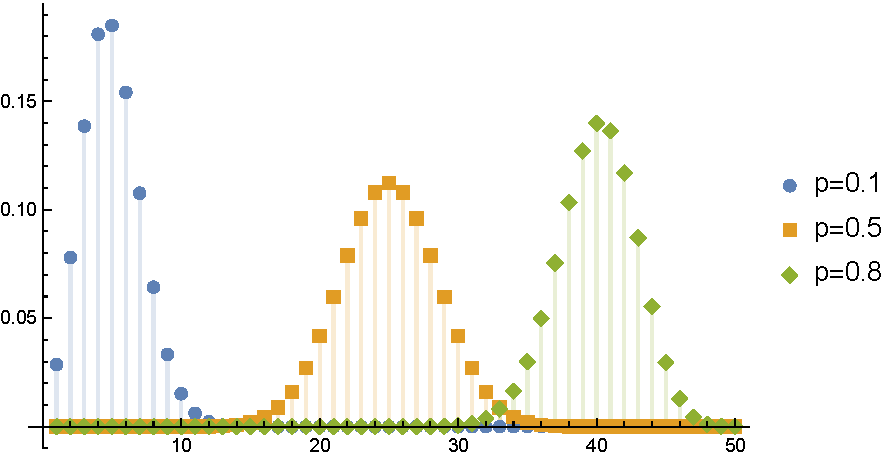
\includegraphics[scale=0.9, center]{images/binomial_distribution.pdf} 
\end{example}

\begin{example}[The Multinomial Distribution]
The multinomial distribution $ \mathcal{M}(\mathbf{x}\,\vert\, n,\mathbf{p})$ is a generalization of the binomial distribution, where the number of possible outcomes is also a variable $m$.  
  \begin{equation}
    \mathcal{M}(x_{1:m}\,\vert\, n,p_{1:m})=\sum_{n_1=0}^n\sum_{n_2=0}^n\ldots \sum_{n_m=0}^n \frac{n!}{n_1!n_2!\ldots n_m!}p_1^{n_1}p_2^{n_2}\ldots p_m^{n_m}\prod_{i=1}^m\delta(x_i-x_{n_i})
  \end{equation}
with the constraints $\sum_{i=1}^{m}n_i=n$ and $\sum_{i=1}^{m}p_i=1$. An application of the multinomial distribution in the context of histograms will be discussed in ~\ref{Histograms}.\\

Wolfram language provides the function \texttt{MultinomialDistribution}

\begin{mathematica}
GraphicsRow[Table[DiscretePlot3D[
   PDF[MultinomialDistribution[n, {0.6, 0.4}], {x, y}],
   {y, 0, n}, {x,0, n}, PlotLabel -> Row[{"n = ", n}], 
   ExtentSize -> 0.5], {n, {3, 6, 9}}], ImageSize -> Full]
\end{mathematica}
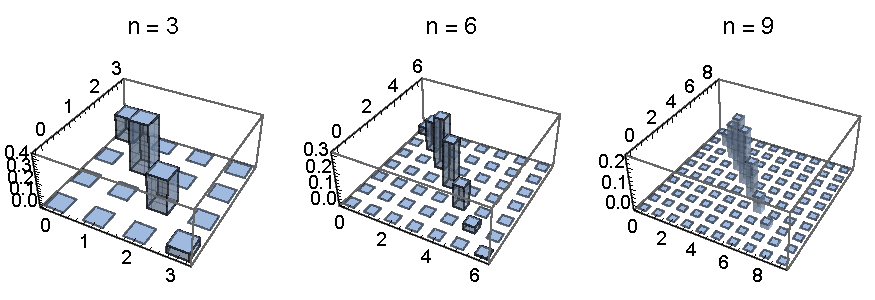
\includegraphics[scale=0.9, center]{images/multinomial_distribution.pdf}  
\end{example}

\begin{example}[The Poisson Distribution]
In the limit $n\rightarrow\infty$ and $\lambda=np$ remains finite, the binomial distribution becomes the Poisson distribution given by
  \begin{equation}
    \mathcal{P}(x\,\vert\,\lambda)=\sum_{k=0}^{\infty}\frac{\lambda^k}{k!}\exp(-\lambda)\delta(x-x_k)
  \end{equation}
 This distribution describes the probability of observing $k$ events given a mean event count of $\lambda$.\\

Wolfram Language has the built-in function \texttt{PoissonDistribution}.
\begin{mathematica}
DiscretePlot[Table[PDF[PoissonDistribution[\[Lambda]], k],
             {\[Lambda], {5, 10, 20}}] // Evaluate,
             {k, 0, 30}, PlotRange -> All, PlotMarkers -> Automatic, 
             PlotLegends -> {"\[Lambda]=5", "\[Lambda]=10", "\[Lambda]=20"}]
\end{mathematica}
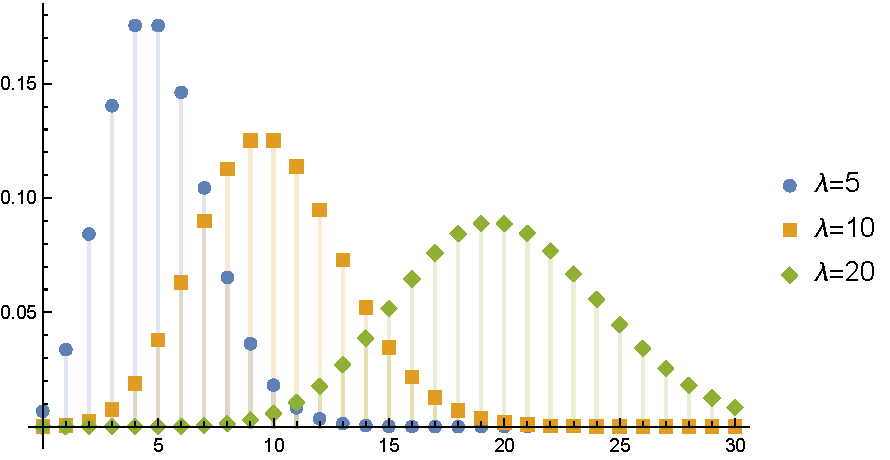
\includegraphics[scale=0.9, center]{images/poisson_distribution.pdf}  
\end{example}

\begin{theorem}[Sum of two Poisson distributions]
  \label{th:sumofpoissondistributions}
  \index{sum of two Poisson distributions}
  Show that $z=x+y$ is distributed as a Poisson-distribution $P(z\,\vert\,\lambda_1+\lambda_2)$ if $y\sim \mathcal{P}(x\,\vert \,\lambda_1)$ and $y\sim \mathcal{P}(y\,\vert \,\lambda_2)$.\\
\end{theorem}
\begin{proof}
  \begin{equation}
    p(z)=\int_{-\infty}^{+\infty}\int_{-\infty}^{+\infty}p(z,x,y)dx dy
    =\int_{-\infty}^{+\infty}\int_{-\infty}^{+\infty}p(z\,\vert\, x,y)\mathcal{P}(x\,\vert\,\lambda_1)\mathcal{P}(y\,\vert\,\lambda_2)dx dy
  \end{equation}
  Bayes rule was used in last step. $p(z\,\vert\, x,y)$ is a deterministic function $z=x+y$ and is given by $\delta\left(z-x-y\right)$. The $y$-integration can be carried out and gives the following result.
  \begin{equation}
    p(z)=\int_{-\infty}^{+\infty}P(x\,\vert\,\lambda_1)P(z-x\,\vert\,\lambda_2)dx
  \end{equation}
  Inserting the expressions for the Poisson distribution and carrying out the $x$-integration leads to
  \begin{equation}
    p(z)=\exp(-\lambda_1-\lambda_2)\sum_{k=0}^{\infty}\frac{\lambda_{1}^k}{k!}\sum_{l=0}^{\infty}\frac{\lambda_{2}^l}{l!}\delta(z-x_k-y_l)
  \end{equation}
  We set now $z_n=x_k+y_l$ with $n=k+l$ by introducing a third sum $\sum_{n=0}^{\infty}\delta_{n,k+l}=1$ and carrying out the summation over $l$   
  \begin{equation}
    p(z)=\exp(-\lambda_1-\lambda_2)\sum_{n=0}^{\infty}\frac{1}{n!}\underbrace{\sum_{k=0}^{n}n!\frac{\lambda_{1}^k}{k!}\frac{\lambda_{2}^{n-k}}{(n-k)!}}_{(\lambda_{1}+\lambda_{2})^n}\delta(z-z_n)
  \end{equation}
  We used here $\delta_{n,k+l}=\delta_{n-k,l}$, which replaces $l$ by $n-k$ and limits the sum over $k$ to $n$, because $l$ is positive and $n-k$ is negative for $k>n$ and the Kronecker delta is therefore always zero.
\end{proof}

In the Wolfram Language the proof is rather simple.
\begin{mathematica}
TransformedDistribution[u + v, 
                        {u \[Distributed] PoissonDistribution[\[Lambda]1],
                         v \[Distributed] PoissonDistribution[\[Lambda]2]}]
\end{mathematica}

\begin{exercise}
   Show that $z_n=\sum_{i=1}^{n}x_i$ is distributed as a Poisson-distribution $P\left(z_n\,\vert\,\sum_{i=0}^n\lambda_i\right)$ if $x_i\sim \mathcal{P}(x_i\,\vert \,\lambda_i)$. Proof this statement by induction using $z_n=z_{n-1}+x_n$. 
\end{exercise}

\begin{exercise}
  Show that the probability density of $z=x+y$ can be written as the convolution of the probability densities of $x$ and $y$.
  \begin{equation}
    p(z)=\int_{-\infty}^{+\infty}p\left(x\right)
    p\left(y=z-x\right)dx
  \end{equation}
  
\end{exercise}

\begin{exercise}
  Show that $z=x+y$ is distributed as 
  $\mathcal{N}\left(z\,\vert\,\mu_1+\mu_2,\sigma_1^2+\sigma_2^2\right)$ if $y\sim \mathcal{N}(x\,\vert \,\mu_1,\sigma_1^2)$ and $y\sim \mathcal{N}(y\,\vert \,\mu_2,\sigma_2^2)$. The first part of the derivation is similar to the one for the Poisson distribution with the result
  \begin{equation}
    p(z)=\int_{-\infty}^{+\infty}\mathcal{N}\left(x\,\vert\,\mu_1,\sigma_1^2\right)
    \mathcal{N}\left(z-x\,\vert\,\mu_2,\sigma_2^2\right)dx
  \end{equation}
  The $x$ integration can be simplified using the variable transformation $x\rightarrow \frac{x-\mu_1-\mu_2}{\sqrt{\sigma_1^2+\sigma_2^2}}$.
\end{exercise}

\section{Expectation, Mean and Variance}

The expectation value of a function $f(x)$ of a random variable $x$, which is distributed as $p(x)$, is defined as
\begin{definition}[Expectation]
  \label{th:expectation}
  \index{expectation}
  \begin{equation}
    \mathbb{E}_{x\sim p(x)}[f(x)]=\int_{-\infty}^{+\infty}f(x) p(x)dx
  \end{equation}
\end{definition}

While the probability density contains all the information needed to perform calculations, it is often useful to characterize its shape by two values: mean and variance.

\begin{definition}[Mean]
  \label{th:mean}
  \index{mean}
  \begin{equation}
    \mu = \mathbb{E}_{x\sim p(x)}[x]=\int_{-\infty}^{+\infty}x p(x)dx
  \end{equation}
\end{definition}

\begin{definition}[Variance]
  \label{th:variance}
  \index{variance}
  \begin{equation}
    \sigma^2=\mathbb{E}_{x\sim p(x)}[(x-\mu)^2]=\int_{-\infty}^{+\infty}(x-\mu)^2 p(x)dx
  \end{equation}
\end{definition}

The normal distribution $\mathcal{N}\left(x\,\vert\, \mu,\sigma^2\right)$ is completely characterized by these values, while other distributions have non-zero expectation value of higher powers of $x-\mu$.\\

Wolfram Language provides the three functions \texttt{Expectation}, \texttt{Mean} and \texttt{Variance}, which can be applied to a distribution e.g. the multi-variate Normal distribution

\begin{mathematica}
Expectation[{x1, x2}, {x1, x2} \[Distributed] 
  MultinormalDistribution[{\[Mu]1, \[Mu]2}, 
                          {{\[CapitalSigma]11, \[CapitalSigma]12},
                           {\[CapitalSigma]12, \[CapitalSigma]22}}]]
Mean[MultinormalDistribution[{\[Mu]1, \[Mu]2}, 
                             {{\[CapitalSigma]11, \[CapitalSigma]12}, 
                              {\[CapitalSigma]12, \[CapitalSigma]22}}]]
Variance[MultinormalDistribution[{\[Mu]1, \[Mu]2}, 
                                 {{\[CapitalSigma]11, \[CapitalSigma]12},
                                  {\[CapitalSigma]12, \[CapitalSigma]22}}]]
\end{mathematica}
The results of these three commands is $\{\mu_1,\mu_2\}$, $\{\mu_1,\mu_2\}$ and $\{\Sigma_{11},\Sigma_{22}\}$.\\

\texttt{Variance} returns only the diagonal elements of the covariance matrix. The function \texttt{Covariance} returns the full covariance matrix.
\begin{mathematica}
Covariance[MultinormalDistribution[{\[Mu]1, \[Mu]2}, 
                                   {{\[CapitalSigma]11, \[CapitalSigma]12},
                                    {\[CapitalSigma]12, \[CapitalSigma]22}}]]
\end{mathematica}
The result is $\begin{pmatrix}\Sigma_{11} & \Sigma_{12} \\
\Sigma_{12} & \Sigma_{22} \\
\end{pmatrix}$.

\begin{example}[Mean and Variance of Poisson Distribution]
What is the mean and variance of a random variable $x$ distributed as a Poisson distribution $\mathcal{P}\left(x\,\vert\,\lambda\right)$ if the possible values $x$ can take are $x_k=k$?\\
The mean $\mu$ is given by 
  \begin{equation}
  \begin{aligned}
    \mu(\lambda)&=\sum_{k=0}^{\infty}P_k k=\sum_{k=1}^{\infty}k\frac{\lambda^k}{k!}\exp(-\lambda)\\ &=\exp(-\lambda)\lambda\sum_{k=1}^{\infty}\frac{\lambda^{k-1}}{(k-1)!}=\exp(-\lambda)\lambda\underbrace{\sum_{k=0}^{\infty}\frac{\lambda^{k}}{k!}}_{\exp(\lambda)}=\lambda
  \end{aligned}
  \end{equation}
The summation range was changed from $k=0$ to $k=1$, because the $k=0$ term is identically zero.\\
The variance $\sigma^2$ can be calculated as 
  \begin{equation}
  \begin{aligned}
    \sigma(\lambda)^2&=\sum_{k=0}^{\infty}P_k (k-\lambda)^2=\sum_{k=0}^{\infty}P_k k^2 - 2\lambda \underbrace{\sum_{k=0}^{\infty}P_k k}_{\lambda} + \lambda^2\underbrace{\sum_{k=0}^{\infty}P_k}_{1}\\
&=\exp(-\lambda)\sum_{k=0}^{\infty}k^2\frac{\lambda^k}{k!} - \lambda^2
  \end{aligned}
  \end{equation}
Applying $\lambda\frac{\partial}{\partial \lambda}$ to $\mu(\lambda)$ gives the following identity
\begin{equation}
\lambda\frac{\partial \mu(\lambda)}{\partial \lambda}=\sum_{k=0}^{\infty}k^2\frac{\lambda^k}{k!}\exp(-\lambda)-\lambda\underbrace{\sum_{k=0}^{\infty}k\frac{\lambda^k}{k!}\exp(-\lambda)}_{\lambda}=\lambda
\end{equation}  
This leads to the final result for $\sigma^2$.
  \begin{equation}
    \sigma(\lambda)^2=\underbrace{\exp(-\lambda)\sum_{k=0}^{\infty}k^2\frac{\lambda^k}{k!}}_{\lambda^2+\lambda} - \lambda^2=\lambda
  \end{equation}  
\end{example}

\begin{exercise}
 Show that the mean and variance of a random variable $x$ distributed as a uniform distribution $\mathcal{U}\left(x\,\vert\,\alpha,\beta\right)$ is given by $\mu=\frac{\alpha+\beta}{2}$ and $\sigma^2=\frac{(\beta-\alpha)^2}{12}$.
\end{exercise}

\section{Examples}

In this chapter we apply the learned concepts to some interesting examples by using both analytical and computational approaches to solve the problem.

\begin{example}[The Monty Hall Problem]

This is a famous and non-trivial example of a probabilistic problem, where intuition will give you the wrong result. The problem statement is as follows:\\

Monty Hall, after which the problem is named, was a moderator of a game show and a participant has to choose between 3 doors. Behind one door a prize is hidden. After the choice has been made e.g. door 2, the moderator opens a door with no prize e.g. door 1, and asks the participant if he wants to choose the remaining door (in this case door 3) or if he wants to stay with his decision (door 2).
\\
\\
\textit{The question is now: What is the probability to win if the participant stays with his first decision or if he chooses the remaining door?}\\

The difficult part is to cast the problem into a manageable form, which means, selecting proper random variables to make the computation as easy as possible. 
A discrete random variable $x_1$ can be associated with the action that the participant chooses a door randomly at the beginning and the choice is either a door with a prize behind it $x_1=p$ or a door with no prize $x_1=n$ (\textit{note that this is not known, when the choice happens, but the crucial point is that the probability for its occurrence can be calculated easily with the result $P(x_1=p)=\frac{1}{3}$ and $P(x_1=n)=\frac{2}{3}$, because there are only 3 doors and one contains a prize and the two others not}).\\ 

Another discrete random variable $x_2$ will be associated with the outcome of the game (participant wins $x_2=w$ or looses $x_2=l$). This is the random variable, which is needed to answer the question above.\\
 
Furthermore we introduce a parameter $\theta$, which describes the two possible ways: participant stays with his first decision ($\theta=0$) or participant chooses the remaining door ($\theta=1$).\\

After the random variables and parameters have been defined, the starting point is always the joint probability $P(x_2,x_1\,\vert\,\theta)$. Because we are only interested in the probability of winning the game, we can marginalize over $x_1$ and use Bayes rule to separate $P(x_1)$, which is known.
  \begin{equation}
    P(x_2=w\,\vert\,\theta)=\sum_{x_1=p,n}P(x_2=w,x_1\,\vert\,\theta)=
    \sum_{x_1=p,n}P(x_2=w\,\vert\,x_1,\theta)P(x_1)
  \end{equation}    
We only need to calculate the conditional probability $P(x_2\,\vert\,x_1,\theta)$. We will see that this quantity is completely deterministic. 
\\
\\
\textit{Let's study first the case $\theta=0$.}\\

In this case if $x_1$ was already the right door with the prize, the participant will win, and if $x_1$ was the wrong door, he will loose regardless if the moderator opens another door without a prize.
  \begin{equation}
   P(x_2\,\vert\,x_1,\theta=0)=
\begin{cases}
1 & x_2=w\:\ \&\:\ x_1=p \\
0 & x_2=l\:\ \&\:\ x_1=p \\
1 & x_2=l\:\ \&\:\ x_1=n \\
0 & x_2=w\:\ \&\:\ x_1=n \\
\end{cases}
  \end{equation}
\\
\\  
\textit{Next we handle the case $\theta=1$.}\\

In this case if $x_1$ was already the right door with the prize, the participant will loose when changing to the remaining door and if $x_1$ was the wrong door, he will win, because the moderator has opened the door without no prize, so the remaining door must contain the prize.
  \begin{equation}
   P(x_2\,\vert\,x_1,\theta=1)=
\begin{cases}
0 & x_2=w\:\ \&\:\ x_1=p \\
1 & x_2=l\:\ \&\:\ x_1=p \\
0 & x_2=l\:\ \&\:\ x_1=n \\
1 & x_2=w\:\ \&\:\ x_1=n \\
\end{cases}                    
  \end{equation}
So the final result is
  \begin{equation}
   P(x_2=w\,\vert\,\theta)=
\begin{cases}
1\cdot\frac{1}{3}+0\cdot\frac{2}{3}=\frac{1}{3} & \theta=0 \\
0\cdot\frac{1}{3}+1\cdot\frac{2}{3}=\frac{2}{3} & \theta=1 \\
\end{cases}
  \end{equation}  
The remarkable result is that making a new choice increases your chances to win considerably. Naively one would have thought that the probability in this case is $\frac{1}{2}$, because after the moderator has opened a door without the prize, two doors are remaining and there is an equal chance to get the right door with the prize. But unfortunately this intuitively convincing argument is wrong.\\

The following code shows a Monte Carlo simulation with the following variables and functions:
\texttt{doorsWithPrize} is a randomly generated list of door numbers, which contain a prize,
\texttt{firstChoice} is a randomly generated list of door numbers from the participant's first choice (this variable will be used to evaluate the case participant stays with his first choice),
\texttt{doorsWithoutPrize} is a randomly generated list of the doors opened by the moderator after the first choice was made,
\texttt{secondChoice} is a list of door numbers from the participant's second choice (this variable will be used to evaluate the case participant chooses the remaining door),
\texttt{ProbabilityWinningPrize} is a function to calculate the probability to win a prize for a given choice (it simply counts the number of elements in the choice list, which agree with the corresponding item in the \texttt{doorsWithPrize} list). 
\\   

\begin{mathematica}
doors = Range[3];
doorsWithPrize = RandomChoice[doors, 1000];
firstChoice = RandomChoice[doors, Length[doorsWithPrize]];
doorsWithoutPrize = MapThread[
                        RandomChoice[Complement[doors, {#1, #2}]] &,
                        {doorsWithPrize, firstChoice}];
secondChoice = MapThread[
                        RandomChoice[Complement[doors, {#1, #2}]] &,
                        {doorsWithoutPrize, firstChoice}];
ProbabilityWinningPrize[choice_] := Apply[Plus, 
                                          MapThread[Boole[#1 == #2] &,
                                          {doorsWithPrize, choice}]
                                          ] / Length[doorsWithPrize] // N;
Print["Probability of winning by staying with your first choice = ", 
      ProbabilityWinningPrize[firstChoice]];
Print["Probability of winning by choosing the remaining door = ", 
      ProbabilityWinningPrize[secondChoice]];
\end{mathematica} 
The probability of winning with 1000 samples is \texttt{0.32} in the case of staying with the first choice and \texttt{0.68} in the case of choosing the remaining door. Using 1000000 samples the values are \texttt{0.333} and \texttt{0.667}, respectively. 
\end{example}

\begin{example}[The Birthday Problem]
The Birthday problem is another classic probabilistic example. Let's assume that each day of the year (we ignore leap years) is equally likely a birthday with probability $p=\frac{1}{365}$. What is the probability that in a group with $n$ distinct individuals (no twins) at least two persons have the same birthday?\\

We want to solve this problem with a simulation and plot the probability as a function of the group size. \\

We create a variable \texttt{birthdays} containing all possible birthdays from \texttt{1} to \texttt{365}.
The main part is the function \texttt{sameBirthdaysInGroup}, which calculates the probability of having at least two persons with the same birthday in a group of $n$ people. A random matrix \texttt{groupSamples} is generated with \texttt{sampleSize} rows and \texttt{n} columns with elements chosen randomly from the list \texttt{birthdays}. The next line evaluates each row of \texttt{groupSamples} if there are same birthdays present. Each row is first sorted and then the difference of each element is calculated. If two birthdays are the same, at least one difference is zero and
\texttt{MemberQ} tests if a zero is present. \texttt{Boole} converts the boolean to numerical values (\texttt{True} to \texttt{1} and \texttt{False} to \texttt{0}) and the result is stored in the variable \texttt{sameBirthDay}. The return value is simply the number of ones in the list \texttt{sameBirthDay} divided by the number of samples.\\ 

\begin{mathematica}
birthdays = Range[365];
SameBirthdaysInGroup[n_Integer] := Module[
   {sameBirthday, groupSamples, sampleSize = 1000},
   groupSamples = RandomChoice[birthdays, {sampleSize, n}];
   sameBirthday = Map[Boole[MemberQ[Differences[Sort[#]], 0]] &, groupSamples];
   Return[Apply[Plus, sameBirthday] / sampleSize // N]
   ];
groupSizes = {5, 10, 15, 20, 25, 30};
probs = Map[SameBirthdaysInGroup, groupSizes];
ListPlot[Transpose[{groupSizes, probs}],
         Filling -> Axis, 
         AxesLabel -> {"n", "Probability"}]
\end{mathematica}

 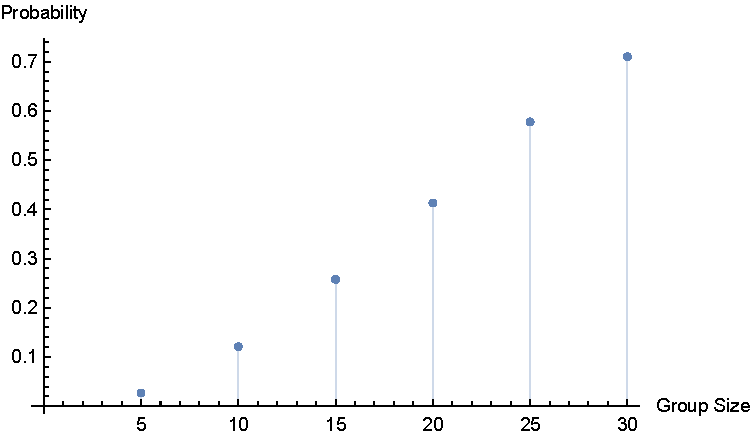
\includegraphics[scale=1, center]{images/double_birthday_problem.pdf}
 
 The probability is larger than 50\%  for a group size > 22.\\

What is the probability that at least three persons have the same birthday?\\

Only one line of the code above has to be changed to answer this question. 
\begin{mathematica}
sameBirthday = 
    Map[Boole[MemberQ[Partition[Differences[Sort[#]], 2, 1], {0, 0}]] &,
    groupSamples];
\end{mathematica}

The function \texttt{Partition} decomposes the differences list into overlapping pairs and any pair with only zeros in it is a triple birthday.\\   

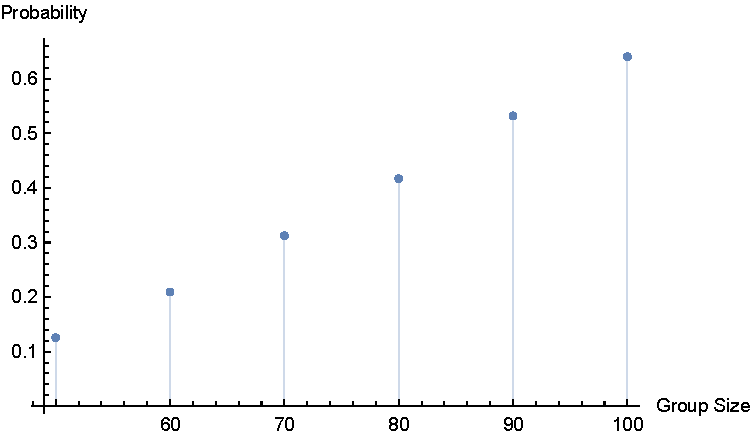
\includegraphics[scale=1, center]{images/triple_birthday_problem.pdf}

So a group of 88 people is needed to have a 50\% chance of having at least three persons with the same birthday.
\end{example}

%---------------------------------------------------------------------------
\chapter{Density Estimation and Random Data}

\begin{summary}
  This chapter deals with the problem how a probability density can be estimated from data and how data can be generated from a distribution.
\end{summary}

\section{Histograms}
\label{Histograms}

A histogram divides the support of a random variable $x$ into disjunct bins and counts the number of outcomes of $x$ in each bin. If $x\sim p(x)$, the normalized count in bin $[x_i,x_{i+1}]$ is given by
  \begin{equation}
    P_i=P\left(x_i\leqq x\leqq x_{i+1}\right)=\int_{x_i}^{x_{i+1}}p(x)dx=\lim_{N\rightarrow\infty}\frac{N_i}{N}
  \end{equation}
The count $N_i$ can only take integer values, therefore $N_i = [P_i N]$, where the symbol $[x]$ means nearest integer of $x$ and $N$ is the total number of outcomes.

Let's assume that we have collected data about the random variable $x$ as $\mathcal{D}=\{x_{1:N}\}$. We assign each data point $x_k$ to a bin and count the number of data points in each bin. If the bins do not cover the whole range of $x$, there will be data points, which can not be assigned to a bin. These data points are called outliers.  

If we represent the bins in terms of a center point $\tilde{x}_i=\frac{x_i + x_{i+1}}{2}$ and the width $w_i=\frac{x_{i+1}-x_i}{2}$, we can write the bin $b_i$ as $[\tilde{x}_i-\frac{w_i}{2},\tilde{x}_i+\frac{w_i}{2}]$.

Then the $N_i$ can be expressed as
  \begin{equation}
    N_i=\sum_{k=1}^{N}\mathcal{I}\left(x_k-\tilde{x}_i;w_i\right)
  \end{equation}
where $\mathcal{I}$ is the indicator function defined as
  \begin{equation}
    \mathcal{I}(x;w)=\begin{cases}1 & x\in [-\frac{w}{2}, +\frac{w}{2}] \\
0 & otherwise \\
\end{cases}
  \end{equation}
Then the probability density estimate $\hat{p}(x)$ can be written as
  \begin{equation}
  \label{eq:probability_density_estimate}
    \hat{p}(x)=\frac{1}{N}\sum_{i=1}^{m}\frac{N_i}{w_i}\mathcal{I}\left(x-\tilde{x}_i;w_i\right)
  \end{equation}
  where $m$ is the number of bins.
  
There are some best practice rules for choosing the number of bins $m$ 
  \begin{equation}
        m = [1 + \log_{2}(N)]
  \end{equation}
and the bin width $w$
  \begin{equation}
        w = 3.5 s N^{-\frac{1}{3}}
  \end{equation}
where $s$ is the standard deviation of the data sample.\\

If we create $n$ histograms from datasets $\mathcal{D}_{1:n}$ sampled from the same distribution $p(x)$ and with the same size $N$, then the bin entries $N_1,N_2,\ldots,N_m$ would be distributed according to a multinomial distribution

  \begin{equation}
    P(N_{1:m}\,\vert\, N,P_{1:m})=\frac{N!}{N_1!N_2!\ldots N_m!}P_1^{N_1}P_2^{N_2}\ldots P_m^{N_m}
  \end{equation}
with $\sum_{i=1}^m N_i=N$ and $P_i$ are the probabilities of $x$ to be assigned to bin $[x_i,x_{i+1}]$.\\

The Wolfram Language provides the function \texttt{Histogram} e.g. 
\begin{mathematica}
Histogram[data, {{1,2,3,4}}]
\end{mathematica}
creates a histogram with 3 bins $[1,2]$, $[2,3]$ and $[3,4]$ or 
\begin{mathematica}
Histogram[data, {-10,10,1}, "Probability"]
\end{mathematica}
creates a histogram of normalized counts $\frac{N_i}{N}$ from $-10$ to $10$ with a bin width of $1$. Using the option \texttt{"PDF"}, a probability density estimate $\hat{p}(x)$ can be plotted. If the bin values and histogram heights are only required numerically, the function \texttt{HistogramList} can be used.\\

A probability density estimate can be constructed with the function \texttt{HistogramDistribution}  according to eq. \ref{eq:probability_density_estimate}.
\begin{mathematica}
data = RandomVariate[NormalDistribution[], 1000];
dist = HistogramDistribution[data];
DiscretePlot[PDF[dist, x], {x, -4, 4, .01}]
\end{mathematica}

 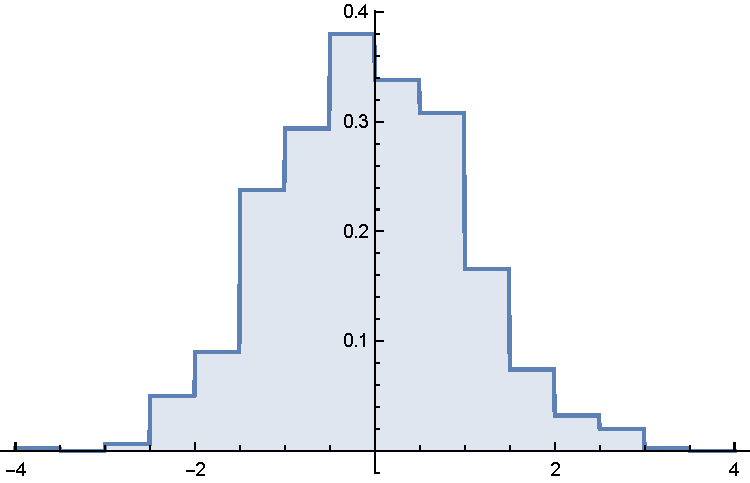
\includegraphics[scale=0.9, center]{images/histogram_distribution.pdf}

In addition, \texttt{Histogram3D} and \texttt{DensityHistogram} are available for bi-variate random data. In the following examples the bi-variate data samples are generated with the \texttt{BinormalDistribution}, which is a special case of the multinormal distribution for $n=2$.

\begin{mathematica}
Histogram3D[RandomVariate[BinormalDistribution[0], 10000]]
\end{mathematica}

 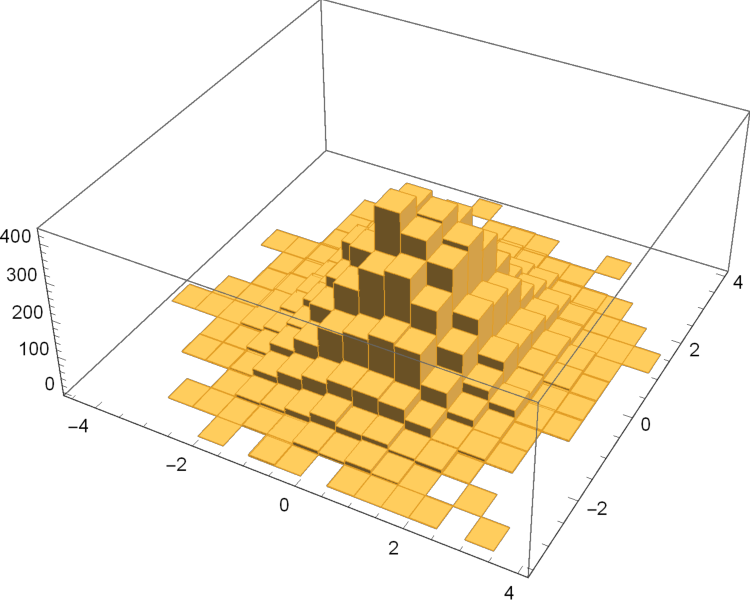
\includegraphics[scale=0.8, center]{images/histogram_3d.pdf}
 
 \begin{mathematica}
DensityHistogram[RandomVariate[BinormalDistribution[0], 10000]]
\end{mathematica}

 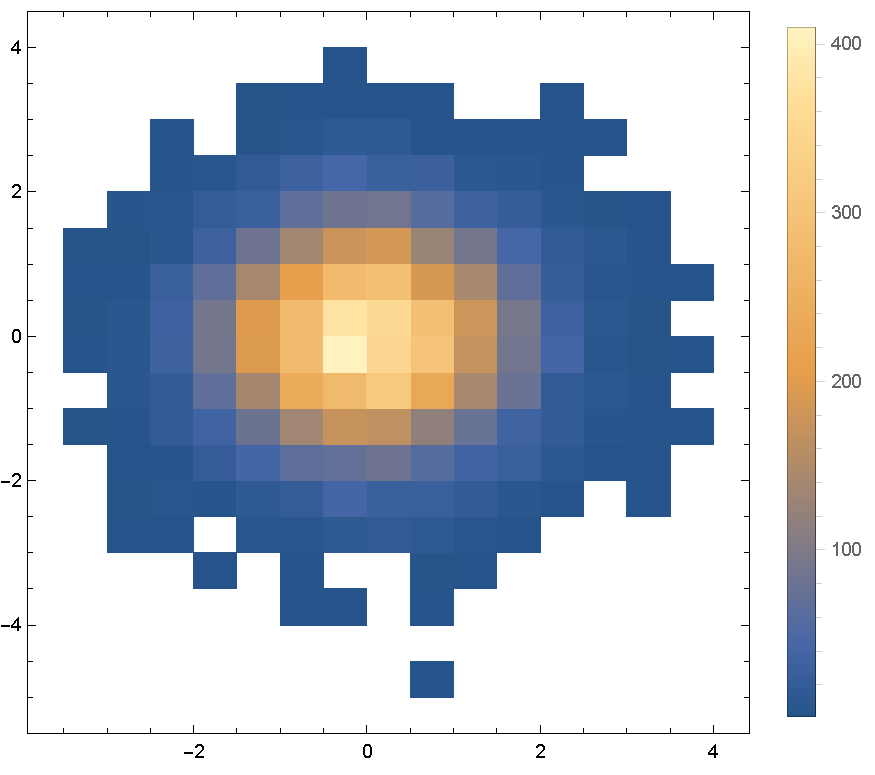
\includegraphics[scale=0.8, center]{images/density_histogram.pdf}     

\begin{exercise}
Verify that $\hat{p}(x)$ given by eq. \ref{eq:probability_density_estimate} is normalized.
  \begin{equation}
\int_{-\infty}^{+\infty}\hat{p}(x)dx=1        
  \end{equation}
\end{exercise}

\section{Gaussian Mixture Model}
Histograms are typically a coarse-grained representation of a probability density, which depends very much on the choice of binning. A better representation is a Gaussian Mixture Model (GMM). 

\begin{definition}[Gaussian Mixture Model]
  \label{th:gaussianmixturemodel}
  \index{gaussian mixture model}
  The Gaussian Mixture Model is defined by
  \begin{equation}
    p_{GMM}(\mathbf{x}\,\vert\,\boldsymbol{\alpha},\boldsymbol{\mu}_{1:N},\boldsymbol{\Sigma}_{1:N}) = \sum_{i=1}^N \alpha_i \mathcal{N}\left(\mathbf{x}\,\vert\,\boldsymbol{\mu}_i,\boldsymbol{\Sigma}_i\right)
  \end{equation}
  with $\sum_{i=1}^N \alpha_i=1$.
\end{definition}

A Gaussian Mixture Model can approximate any continuous probability density as long as $N$ is big enough.\\

Wolfram Language can learn GMM's from data using the high-level function \texttt{LearnDistribution} with the option \texttt{Method -> "GaussianMixture"}.

\begin{mathematica}
mixture = MixtureDistribution[{0.4, 0.6},
             {NormalDistribution[], NormalDistribution[2, 0.5]}];
data = RandomVariate[mixture, 1000];
dist = LearnDistribution[data, Method -> "GaussianMixture"];
Plot[{PDF[dist, x], PDF[mixture, x]}, {x, -4, 4},
     Filling -> Axis, 
     PlotLegends -> Placed[{"Data", "GMM"}, Right] 
\end{mathematica}

 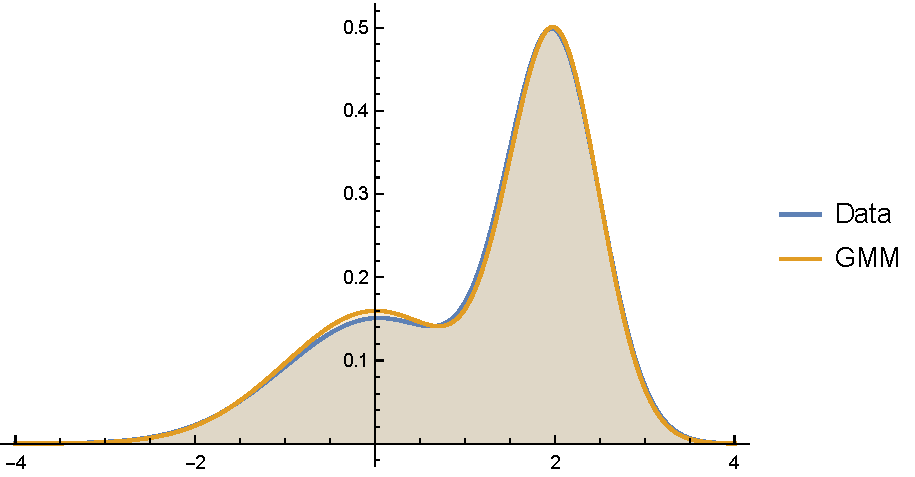
\includegraphics[scale=0.9, center]{images/gaussian_mixture_model.pdf}   

 
\section{Maximum Likelihood}
If the physical process how data is generated is understood, the functional form of the probability density $p(\mathbf{x}\vert \boldsymbol{\theta})$ is typically known. In these cases the goal is to estimate the parameters $\boldsymbol{\theta}$ of a probability density from data.

\begin{definition}[Likelihood]
  \label{th:likelihood}
  \index{likelihood}
  The likelihood is defined by
  \begin{equation}
    \mathcal{L}(\boldsymbol{\theta}) = \prod_{i=1}^N p\left(x_i\,\vert\, \boldsymbol{\theta}\right)
  \end{equation}
where $x_i \in \mathcal{D}=\{x_{1:N}\}$. It is a function of the parameter of the probability density, not a distribution.
\end{definition}
Using the logarithm of the likelihood is better from the view point of numerical stability. 
\begin{definition}[Loglikelihood]
  \label{th:loglikelihood}
  \index{loglikelihood}
  The loglikelihood is defined by
  \begin{equation}
    \log(\mathcal{L}(\boldsymbol{\theta})) = \sum_{i=1}^N \log\left(p\left(x_i\,\vert\, \boldsymbol{\theta}\right)\right)
  \end{equation}
\end{definition}
An optimal estimate of the parameters $\boldsymbol{\hat{\theta}}$ can be found by solving 
$\frac{ \partial\log\left(\mathcal{L}(\boldsymbol{\theta})\right)}{\partial\boldsymbol{\theta}}=0$. The probability density $p(\mathbf{x}\vert \boldsymbol{\hat{\theta}})$ is then called the Maximum Likelihood estimate. 

\begin{example}[Parameter Estimation of Normal Distribution]
The loglikelihood function for the Normal distribution is given by
  \begin{equation}
    \log(\mathcal{L}(\mu,\sigma^2) = \sum_{i=1}^N \log\left(\mathcal{N}\left(x_i\,\vert\, \mu,\sigma^2\right)\right)
  \end{equation}
Inserting the function form of $\mathcal{N}\left(x\,\vert\, \mu,\sigma^2\right)$ gives the following expression
  \begin{equation}
    \log(\mathcal{L}(\mu,\sigma^2) = \frac{1}{2\sigma^2}\sum_{i=1}^N \left(x_i-\mu\right)^2+\frac{N}{2}\log\left(2\pi\sigma^2\right)
  \end{equation}   
The derivative with respect to $\mu$ gives
  \begin{equation}
    \frac{\partial\log(\mathcal{L}(\mu,\sigma^2)}{\partial\mu} = -\frac{1}{\sigma^2}\sum_{i=1}^N \left(x_i-\mu\right)= -\frac{1}{\sigma^2}\left(\sum_{i=1}^N x_i - N\mu\right)=0
  \end{equation}
and has the solution $\hat{\mu}=\frac{1}{N}\sum_{i=1}^N x_i$ (sample mean).\\

The derivative with respect to $\sigma^2$ gives
  \begin{equation}
    \frac{\partial\log(\mathcal{L}(\mu,\sigma^2)}{\partial\sigma^2} = -\frac{1}{2\sigma^4}\sum_{i=1}^N \left(x_i-\mu\right)^2 + \frac{N}{2\sigma^2}=-\frac{1}{2\sigma^4}\left(\sum_{i=1}^N \left(x_i-\mu\right)^2 - N\sigma^2\right)=0
  \end{equation}
and has the solution $\hat{\sigma}^2=\frac{1}{N}\sum_{i=1}^N \left(x_i-\hat{\mu}\right)^2$ (biased sample variance). An unbiased sample variance is given by $s^2=\frac{1}{N-1}\sum_{i=1}^N \left(x_i-\hat{\mu}\right)^2$.
 
\end{example} 

Wolfram Language has built in Maximum Likelihood parameter estimation using the function \texttt{EstimatedDistribution} with the option \texttt{ParameterEstimator -> "MaximumLikelihood"}.

\begin{mathematica}
data = RandomVariate[NormalDistribution[0, 1], 1000];
dist = EstimatedDistribution[data, NormalDistribution[\[Mu], \[Sigma]],
                             ParameterEstimator -> "MaximumLikelihood"]
\end{mathematica}
has the result \texttt{NormalDistribution[0.0400075, 0.974344]}.
\begin{mathematica}
{Mean[data], StandardDeviation[data], RootMeanSquare[data - Mean[data]]}
\end{mathematica}
has the result \texttt{\{0.0400075, 0.974832, 0.974344\}}. The function 
\texttt{StandardDeviation} implements the square root of the unbiased sample variance, while \texttt{RootMeanSquare[data - Mean[data]]} calculates the square root of the biased sample variance, which agrees with the result from the Maximum Likelihood calculation.\\

The function \texttt{FindDistribution} tries to find the best distribution for the given data.
\begin{mathematica}
FindDistribution[data]
\end{mathematica}
returns exactly the same result as the Maximum Likelihood estimator without specifying a distribution as an argument.

\begin{example}[Parameter Estimation of Poisson Distribution]
In the case of a discrete probability density like the Poisson distribution, the likelihood is calculated with the probabilities evaluated on the data samples $x_{1:N}$.
  \begin{equation}
    \mathcal{L}(\lambda) = \prod_{i=1}^N \frac{\lambda^{x_k}}{x_k!}\exp{(-\lambda)}= \frac{\lambda^{\sum_{i=1}^N x_k}}{\prod_{i=1}^N x_k!}\exp{(-N\lambda)}
  \end{equation}
Differentiating with respect to $\lambda$ gives
  \begin{equation}
    \frac{\partial\mathcal{L}(\lambda)}{\partial\lambda} = \left(\frac{\sum_{i=1}^N x_k}{\lambda} - N\right)\frac{\lambda^{\sum_{i=1}^N x_k}}{\prod_{i=1}^N x_k!} \exp{(-N\lambda)} =0
  \end{equation}
The result is $\hat{\lambda} = \frac{1}{N}\sum_{i=1}^N x_k$ (sample mean).
\end{example}


\begin{exercise}
The likelihood of a uniform distribution evaluated on the data samples $x_{1:N}$ is given by
  \begin{equation}
  \label{eq:uniform_likelihood}
    \mathcal{L}(\alpha,\beta) = \prod_{i=1}^N \frac{1}{\beta-\alpha}\Theta(x_k-a)\Theta(b-x_k)= \frac{1}{(\beta-\alpha)^N}\Theta(x_{min}-\alpha)\Theta(\beta - x_{max})
  \end{equation}
with $x_{min} = \text{min}(x_{1:N})$ and $x_{max} = \text{max}(x_{1:N})$. Show that eq. \ref{eq:uniform_likelihood} has a maximum at $\alpha = x_{min}$ and $\beta = x_{max}$.
\end{exercise}

\section{Sampling}
In the previous sections we studied the reconstruction of a probability density from data. Here we investigate the inverse problem: the generation of data from a given probability density. This process is called sampling.

It is usually quite easy to generate random numbers $r$ from a uniform distribution $\mathcal{U}(r\,\vert\,\alpha=0,\beta=1)$. Almost every programming language has a function for it (in the Wolfram Language the function is called \texttt{RandomReal}) . The goal is now to transform the sequence $r_{1:N}$ to a sequence $x_{1:}$ so that $x$ is distributed as $p(x)$.

One way to do this is to find a transformation function $x(r)$ for $0\leqq r \leqq 1$.

\begin{equation}
  \Phi(x(r))=\int_{-\infty}^{x(r)}p(x)dx = \int_{-\infty}^{r}\mathcal{U}(r=r'\,\vert\,\alpha=0,\beta=1)dr'=r
\end{equation}
$\Phi(x)$ is the cumulative distribution function (see \ref{th:cumulativedistributionfunction}) evaluated at $x(r)$. Therefore the function $x(r)$ is the inverse of the cdf evaluated at $r$.
\begin{equation}
  x(r) = \Phi^{-1}(r)
\end{equation}

\begin{example}[Sampling from a Discrete Distribution]
Let's assume that we have an array of probabilities $P_{1:N}$ with $\sum_{i=1}^{N}P_i=1$ and we want to sample an index variable $j\in [1,2,\ldots,N]$ from this distribution.\\

In this case the cumulative distribution is given by $\Phi(j)=\sum_{i=1}^{j}P_i$, where the index $j$ has a range from $0$ to $N$ and $\Phi(0)=0$.
We iterate the index $j$ from $N$ down to $0$ and stop as as soon as the condition $\Phi(j) < r$ is fulfilled. Finally we increment the index $j\rightarrow j+1$, because the possible value range of $j$ is from $0$ to $N-1$ and we need to map them to the range from $1$ to $N$. This procedure generates an index sequence with the desired distribution.\\

The Wolfram Language provides the function \texttt{EmpiricalDistribution} to construct a pdf from a list of weights, which need not to be normalized. Using \texttt{RandomVariate} 1000 samples are drawn from this pdf and are used to fill a histogram.
 
\begin{mathematica}
weights = {200, 300, 200, 100, 200};
categories = Range[1, Length[weights]];
dist = EmpiricalDistribution[weights -> categories];
data = RandomVariate[dist, 1000];
Histogram[data,
          LabelingFunction -> Center,
          AxesLabel -> {"Category", "Count"}]
\end{mathematica}

The histogram shows the counts of the data samples generated from an empirical distribution for each category. The counts are indeed numerically close to the given weights.\\

 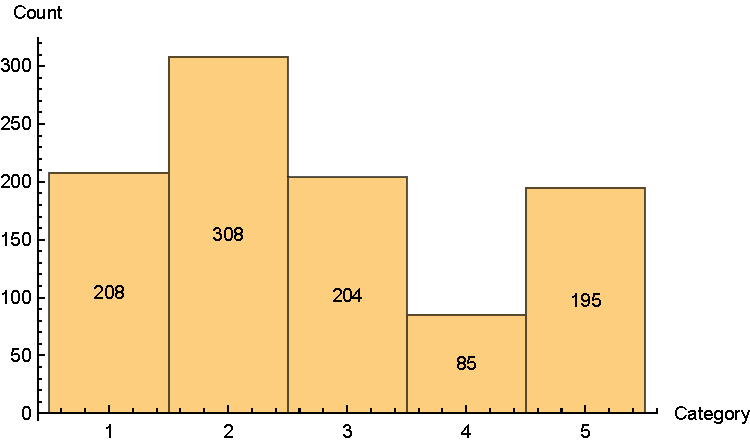
\includegraphics[scale=1, center]{images/sampling_from_discrete_distribution.pdf}   
\end{example}

\begin{example}[Sampling from a Histogram]
If the probability density is given as a histogram, the sampling procedure is the following:
\begin{itemize}
\item Sample a bin index $j$ using the bin heights $\frac{N_i}{N}$ as you would sample from a discrete distribution.
\item Sample $x$ from a uniform distribution $\mathcal{U}\left(x\,\vert\,\alpha=\tilde{x}_j-\frac{w_j}{2},\beta=\tilde{x}_j+\frac{w_j}{2}\right)$.
\end{itemize}
where $\tilde{x}_j$ is the center coordinate and $w_j$ is the width of bin $j$.\\

The Wolfram Language provides the function \texttt{HistogramDistribution}, which can be constructed from given data and can be also used to generate new data samples using \texttt{RandomVariate}, but we first we want to implement our own function based on the sampling procedure described above. \\

The function \texttt{SampleFromHistogram} has three arguments: the bin interval limits \texttt{bins} as a list of $N+1$ elements, the normalized bin heights \texttt{binHeights} as a list with $N$ elements and the number of samples \texttt{numSamples}. So the number of bins $N$ is provided implicitely by the length of the list arguments. It calculates first the cumulative sum of the bin heights, where zero is appended at the beginning of the list. \texttt{numSamples} random numbers are generated to sample a list of bin indices. This is done by subtracting the random number from each element of the cumulative sum and keep only the largest element of the non-positive results. The index is then used to generate uniformly distributed random numbers inside the corresponding bin.
\begin{mathematica}
SampleFromHistogram[bins_, binHeights_, numSamples_] := Module[
  {cumSum, randomNumbers, binIndices, histSamples},
  cumSum = Prepend[Accumulate[binHeights], 0];
  randomNumbers = RandomReal[1, numSamples];
  binIndices = Flatten[Map[Ordering[Select[cumSum - #, NonPositive], -1] &, 
                           randomNumbers]];
  histSamples = Map[RandomReal[{bins[[#]], bins[[# + 1]]}] &, binIndices];
  Return[histSamples]]

data = SampleFromHistogram[{1, 3, 5, 10, 12},
                           {0.1, 0.2, 0.5, 0.2}, 
                           1000];
Histogram[data, {{1, 3, 5, 10, 12}}, "Probability"]    
\end{mathematica}
 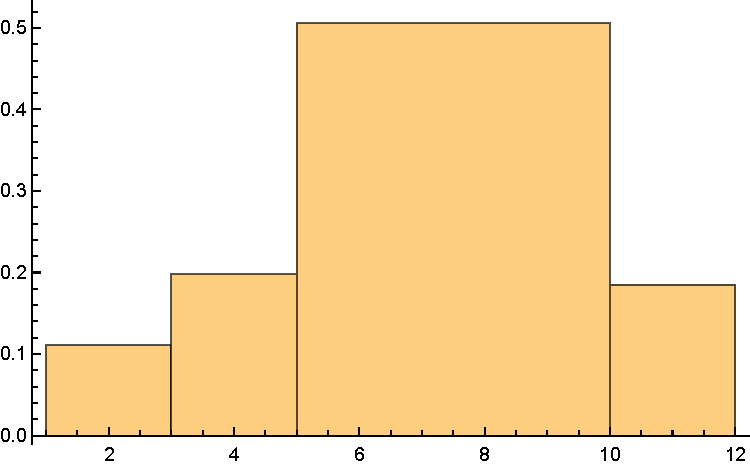
\includegraphics[scale=0.9, center]{images/histogram_sampling.pdf}   

The same result can be obtained with
\begin{mathematica}
dist = HistogramDistribution[data, {{1, 3, 5, 10, 12}}];
data2 = RandomVariate[dist, 1000];
Histogram[data2, {{1, 3, 5, 10, 12}}, "Probability"]
\end{mathematica}
but the performance is much better (almost a factor 100 using \texttt{Timing} to measure the runtime of \texttt{SampleFromHistogram} and \texttt{RandomVariate} generating 1000000 samples). 
\end{example}

\begin{example}[Normal-Distributed Random Numbers]
The trick here is to perform the transformation on the joint pdf of $x$ and $y$, where both random variables are identically distributed according to $\mathcal{N}(\_\,\vert\,\mu=0,\sigma^2=1)$.
\begin{equation}
  \int_{-\infty}^{+\infty}\int_{-\infty}^{+\infty}\mathcal{N}(x\,\vert\,\mu=0,\sigma^2=1)\mathcal{N}(y\,\vert\,\mu=0,\sigma^2=1)dxdy=1
 \end{equation}
 Using the transformation $x=\rho\cos(\phi)$ and $y=\rho\sin(\phi)$, the double integral can written as
\begin{equation}
   \frac{1}{2\pi}\int_{0}^{2\pi}d\phi\int_{0}^{+\infty}\exp\left(-\frac{\rho^2}{2}\right)\rho d\rho=
   \int_{0}^{1}d\phi'\int_{0}^{+\infty}\exp\left(-\rho'\right)d\rho'=1
 \end{equation}
 where the new variables $\rho'$ and $\phi'$ are given by $\rho'=\frac{\rho^2}{2}$ and $\phi'=\frac{\phi}{2\pi}$. So $\phi'$ is uniformly distributed in the range $[0,1]$ and $\rho'$ is exponentially distributed with $\xi=1$.\\

We leave it as an exercise to show that $\rho'(r)=-\log
\left(r\right)$ and therefore $\rho(r)=\sqrt{-2\ln\left(r\right)}$.\\

The transformation function for $\phi$ is given by $\phi(r)=2\pi r$. Because $\phi$ and $\rho$ are independent random variables, we must also use independent random number sequences $r$ and $s$ to evaluate them.\\

Therefore the transformation for $x$ is given by
\begin{equation}
x(r,s)=\sqrt{-2\ln(r)}\cos(2\pi s)
 \end{equation}
 and for $y$ by
 \begin{equation}
y(r,s)=\sqrt{-2\ln(r)}\sin(2\pi s)
 \end{equation}
The algorithm is called Box-Muller method \cite{box1958}.
\end{example}

Random numbers can be generated with the Wolfram Language using \texttt{RandomVariate} for any built-in distribution e.g.

\begin{mathematica}
data1 = RandomVariate[NormalDistribution[0, 1], 1000];
data2 = RandomVariate[NormalDistribution[2, 0.5], 1000];
Histogram[{data1, data2}]
\end{mathematica}

 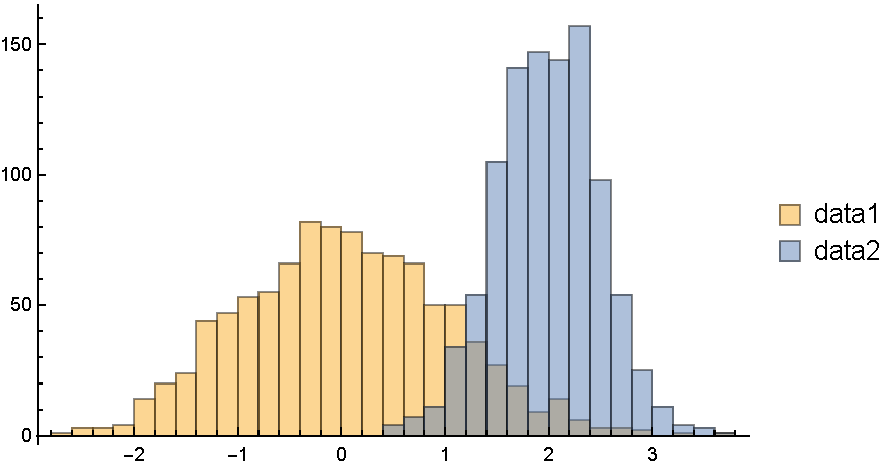
\includegraphics[scale=1, center]{images/normal_distributions_from_data.pdf}
   
\begin{exercise}
  Show that the function $x(r)$ for the exponential distribution 
  $p(x)=\frac{1}{\xi}\exp\left(-\frac{x}{\xi}\right)$ is given by $x(r)=-\xi\ln\left(1-r\right)$ or $x(r)=-\xi\ln\left(r\right)$.   
\end{exercise}

\begin{exercise}
  Show how the method above can be extended to generate random numbers distributed as $\mathcal{N}(\_\,\vert\,\mu,\sigma^2)$.   
\end{exercise}

Finding a function $x(r)$ analytically is not always possible. Another approach, which is applicable to a wider range of distributions, is rejection sampling \cite{neumann1951}. 
\begin{definition}[Rejection Sampling]
  \label{th:rejectionsampling}
  \index{rejection sampling}
The algorithm works in the following way:
\begin{itemize}
\item
Choose a number $M$ and a distribution $p(y)$ in such a way that the condition $p(x=u)\leqq M p(y=u)$ holds everywhere on the support of $x$ and drawing samples from $p(y)$ is known. 
\item 
Draw samples $y_k$ from a distribution $p(y)$ and $r_k$ from a uniform distribution $\mathcal{U}(r\,\vert\,\alpha=0,\beta=1)$ for $k=1:N$.
\item
Check for all $k$ the condition $r_k < \frac{p(x=y_k)}{M p(y=y_k)}$. If it is true, accept $y_k$ as a sample from $p(x)$, otherwise reject the sample.
\end{itemize}
\end{definition}
If $p(x)$ is bounded to a finite interval $[a,b]$, the algorithm can be simplified:
\begin{itemize}
\item
Choose $p_{max}$ as the maximum value of $p(x)$ for $x\in [a,b]$
\item 
Draw samples $x_k=(b-a)s_k+a$ from a uniform distribution $\mathcal{U}(s\,\vert\,\alpha=0,\beta=1)$ and $r_k$ from a uniform distribution $\mathcal{U}(r\,\vert\,\alpha=0,\beta=1)$ for $k=1:N$.
\item
Check for all $k$ the condition $r_k < \frac{p(x=x_k)}{p_{max}}$. If it is true, accept $x_k$ as a sample from $p(x)$, otherwise reject the sample.
\end{itemize}
The rejection rate determines the efficiency of the algorithm.

\begin{example}[Sampling from a SemiCircle Distribution]
We want to sample data from a semicircle distribution

\begin{equation}
p(x)=\begin{cases}\frac{2}{\pi}\sqrt{1-x^2} & -1 \leqq x \leqq +1 \\
0 & otherwise \\
\end{cases}
\end{equation}
The maximum value of the distribution is given by $p_{max}=\frac{2}{\pi}$.\\

The following Wolfram language code implements rejection sampling for this distribution.
\begin{mathematica}
pmax = 2/Pi;
SemiCircleDistribution[x_] := pmax * Sqrt[1 - x^2];
xk = RandomVariate[UniformDistribution[{-1, 1}], 10000];
rk = RandomVariate[UniformDistribution[{0, 1}], 10000];
data = Pick[xk, MapThread[#1 < (SemiCircleDistribution[#2]/pmax) &, {rk, xk}]];
Show[{Histogram[data, 20, "PDF"], 
      Plot[SemiCircleDistribution[x], {x, -1, 1}]}]
\end{mathematica}

 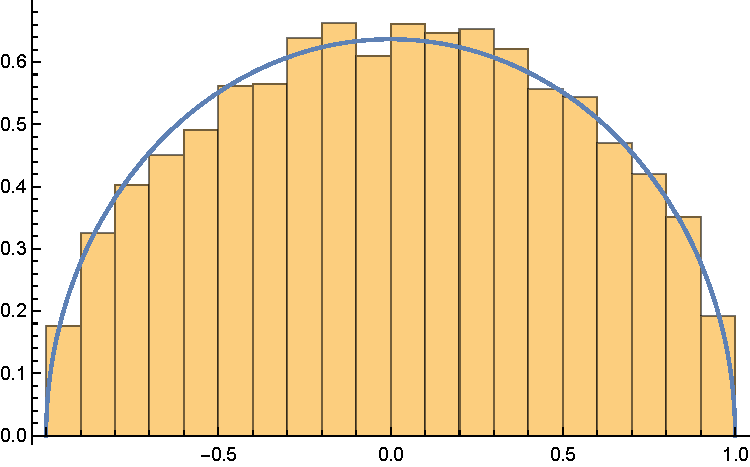
\includegraphics[scale=0.9, center]{images/rejection_sampling.pdf}

\end{example} 

\begin{example}[Sampling from a Gaussian Mixture Model]
Sampling from a Gaussian Mixture Model is easy to implement in the Wolfram Language. We write a function \texttt{SampleFromGaussianMixtureModel} with four arguments: \texttt{weights}, which are the normalized coefficients as a list, \texttt{means}, which is a list of mean vectors or numbers, \texttt{covariances}, which is a list of covariance matrices or standard variances and \texttt{numSamples}, which is the number of samples, which should be returned. In the case of a multi-variate distribution, the returned samples are a matrix with \texttt{numSamples} rows and as many columns as there are variables. The first step is to create a list of normal distributions with the parameters specified by \texttt{means} and \texttt{covariances}, which will be the input for the \texttt{MixtureDistribution} together with \texttt{weights}. This gives already a distribution, where we can sample from using \texttt{RandomVariate}.
The output will be either a list of samples in the uni-variate case or a matrix with \texttt{numSamples} and as many columns as there are variables in the multi-variate case.
  
\begin{mathematica}
SampleFromGaussianMixtureModel[weights_,
                               means_,
                               covariances_,
                               numSamples_] := Module[
  {distributions, mixture, samples},
  distributions = If[NumberQ[means[[1]]],
                     MapThread[NormalDistribution[#1, #2] &,
                               {means, covariances}],
                     MapThread[MultinormalDistribution[#1, #2] &,
                               {means, covariances}]];
  mixture = MixtureDistribution[weights, distributions];
  samples = RandomVariate[mixture, numSamples];
  Return[samples]]
  
data = SampleFromGaussianMixtureModel[{0.3, 0.7}, 
                                      {1, 2}, {1, 1}, 
                                      1000];
Show[{Histogram[data, 20, "PDF"], 
      Plot[{0.3 * PDF[NormalDistribution[1, 1], x],
            0.7 * PDF[NormalDistribution[2, 1], x], 
            0.3 * PDF[NormalDistribution[1, 1], x] + 
            0.7 * PDF[NormalDistribution[2, 1], x]}, {x, -2, 5}]}] 
\end{mathematica}

 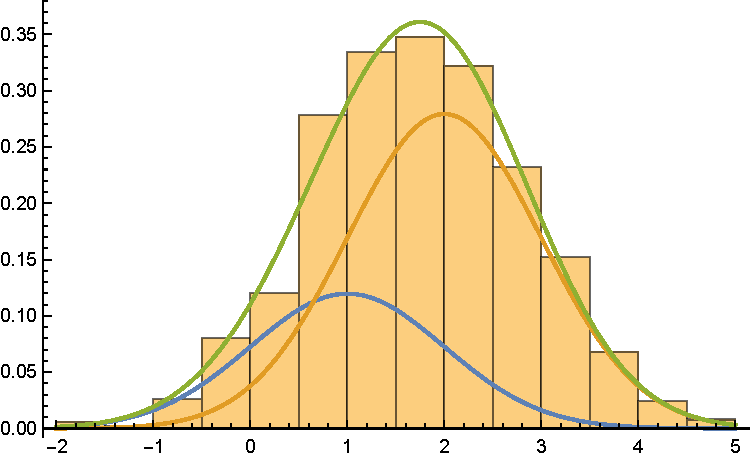
\includegraphics[scale=0.9, center]{images/gaussian_mixture_model_sampling.pdf}
\end{example}

%---------------------------------------------------------------------------
\chapter{Probabilistic Models (Theory)}

\begin{summary}
  This chapter introduces the theoretical foundations of probabilistic models, especially how models can be decomposed into simpler parts and how these parts are connected with each other. Such structures can be best represented by graphs or networks, which allows us to identify important relations between random variables. These graphical representations help us also to deal systematically with more complex and diverse systems and allow us to formulate and implement everything in a common graphical way built on top of graph theory, which provides us with mathematical algorithms to perform efficient calculations.
\end{summary}

\section{Graphical Models}

Probabilistic models are described by a number of random variables $x_{1:n}$, a number of parameters $\theta_{1:m}$ and a joint probability density $p(x_{1:n}\,\vert\, \theta_{1:m})$. It is often favorable to introduce further hidden or latent variables $h_{1:k}$, which are not directly observable and therefore do not show up as inputs or outputs of the system, but are hidden inside the model.
\begin{equation}
p(x_{1:n}\,\vert\, \theta_{1:m})=\int_{-\infty}^{+\infty}dh_{1}\ldots \int_{-\infty}^{+\infty}dh_{k} p(x_{1:n},h_{1:k}\,\vert\, \theta_{1:m})
\end{equation}
These new variables $h_{1:k}$ encode some static or dynamic properties of the system state and often simplify the overall structure of the model by decoupling the outputs from the inputs, which reduces the dependencies between the random variables and parameters in the model. Dependency or causal relations can be very vividly expressed through a graph. Such a graph is also called a belief or Bayesian network \cite{barber2011} \cite{koller2009}.

\begin{definition}[Belief Network]
  \label{th:beliefnetwork}
  \index{belief network}
  A belief network is a directed graph of random variables $x_{1:n}$, which represents a probability distribution of the form
  \begin{equation}
    p(x_{1:n})=\prod_{i=1}^{n}p\left(x_i\,\vert\, pa(x_i)\right)
  \end{equation}
  where $pa(x_i)$ are all random variables $x_j$ (parents), which are connected to the random variable $x_i$ (child) with a directed edge pointing from node $x_j$ to node $x_i$.
\end{definition}

The following Wolfram Language code draws a graph with 3 random variables $x$, $y$, $z$ and one parameter $\theta$. The function \texttt{Graph} gets an adjacency list as the first argument, which contains a list of edges. The nodes or vertices are numbered from $1$ to $4$ and \texttt{i \textbackslash\lbrack DirectedEdge\rbrack \,j} means that there is a directed edge from node $i$ to $j$. This expresses a conditional dependence of node $j$ on node $i$. The other options are only necessary to customize the graphical representation.\\

\begin{mathematica}
Graph[{1 \[DirectedEdge] 3, 2 \[DirectedEdge] 3, 4 \[DirectedEdge] 3},
      VertexLabels -> {1 -> "x", 2 -> "y", 
                       3 -> Placed["z", Below], 4 -> \[Theta]},
      VertexShapeFunction -> {4 -> "Square"}, VertexSize -> Tiny]
\end{mathematica}
 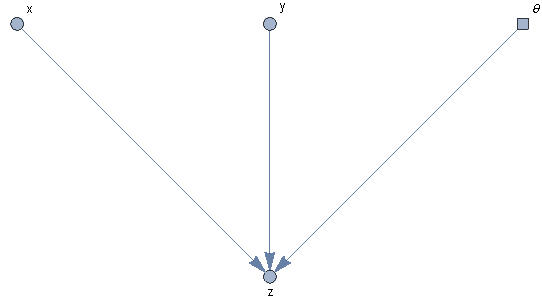
\includegraphics[scale=0.9, center]{images/simple_graph.pdf}

From this graph we can immediately derive the joint probability density as
\begin{equation}
\label{eq:belief}
p(x,y,z\,\vert\, \theta)=p(z\,\vert\, x,y,\theta)p(x)p(y)
\end{equation}

The multivariate probability density is decomposed into univariate probability densities. We saw such a decomposition already in eq. \ref{eq:decomposition}. We can iteratively apply Bayes rule to $p(x,y,z\,\vert\, \theta)$ with the result

\begin{equation}
\begin{aligned}
p(x,y,z\,\vert\, \theta)&=p(z\,\vert\, x,y,\theta)p(y\,\vert\, x,\theta)p(x\,\vert\, \theta)\\
p(x,y,z\,\vert\, \theta)&=p(x\,\vert\, y,z,\theta)p(z\,\vert\, y,\theta)p(y\,\vert\, \theta)\\
p(x,y,z\,\vert\, \theta)&=p(y\,\vert\, z,x,\theta)p(x\,\vert\, z,\theta)p(z\,\vert\, \theta)\\
\end{aligned}
\end{equation}

and the corresponding graphs

 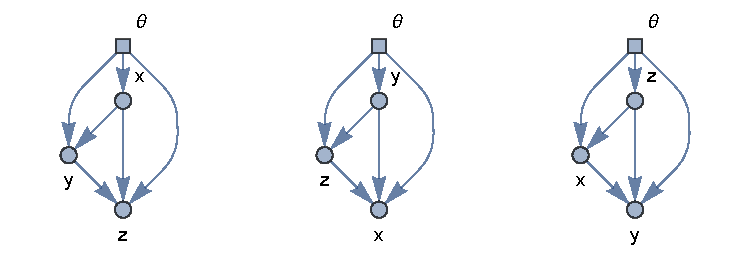
\includegraphics[scale=0.9, center]{images/decomposition_graphs.pdf}

All these decompositions are equivalent and differ only by a reordering of the random variables $x$, $y$ and $z$. The first one can be rewritten to eq. \ref{eq:belief} using $p(y\,\vert\, x,\theta)=p(y)$ and $p(x\,\vert\, \theta)$ assuming that $y$ is conditionally independent of $x$ and $\theta$ and $x$ is conditionally independent of $\theta$, but the other two decompositions seem to express contradictory conditional independence relations, so what is now correct?\\

One has to be careful to interpret these equations as conditional independence relations e.g. the third equation has a term $p(z\,\vert\, \theta)$, which indicates that $z$ is only conditionally dependent on $\theta$, which could be right or wrong. This can be only decided if the probability density is known. If it is right, $p(z\,\vert\, \theta)$ can indeed be written as a function of the parameter $\theta$ only. If it is wrong e.g. $z$ depends on $x$ and $y$, $p(z\,\vert\, \theta)$ is the result of a marginalization of $\int_{-\infty}^{+\infty}\int_{-\infty}^{+\infty}p(z\,\vert\, x,y,\theta)p(x)p(y)dxdy$.\\

The graph does exactly that: it specifies conditional independence relations through the lack of edges between certain nodes (in the example above the edges $\theta\rightarrow x$, $\theta\rightarrow y$ and $x\rightarrow y$) , which can be used to simplify the joint probability density. This is basically an assumption or belief based on some prior knowledge. If this assumption is valid or sufficient to describe the observations or data, has to be verified.\\
 
Using eq. \ref{eq:belief} it can be easily shown that $x$ and $y$ are independent.

\begin{equation}
p(x,y\,\vert\,\theta)=\int_{-\infty}^{\infty}dz p(x,y,z\,\vert\,\theta)=\int_{-\infty}^{\infty}dz p(z\,\vert\, x,y,\theta)p(x)p(y) = p(x)p(y)
\end{equation}
This independence relation holds for any subgraph of the form

 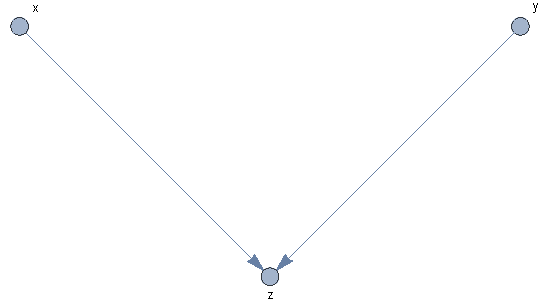
\includegraphics[scale=0.7, center]{images/v_structure.pdf}

which is also called v-structure.

\begin{remark}
Note that $x$ and $y$ in the v-structure are not conditionally independent given $z$.
\begin{equation}
p(x,y\,\vert\,z)=\frac{p(x,y,z)}{p(z)}=\frac{p(z\,\vert\, x,y)p(x)p(y)}{p(z)}
\end{equation}
\end{remark}

\begin{example}
\label{ex:chain_graph}
Show that the graph
 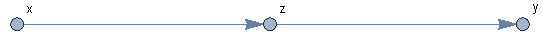
\includegraphics[scale=0.8, left]{images/graph_example.pdf}
 implies the independence of $x$ and $y$ given $z$.\\
 
 The joint probability density for this graph is given by
\begin{equation}
p(x,y,z)=p(y\,\vert\,z)p(z\,\vert\,x)p(x)=p(y\,\vert\,z)p(z,x)=p(y\,\vert\,z)p(x\,\vert\,z)p(z)
\end{equation}
Therefore we get for $p(x,y\,\vert\,z)$
\begin{equation}
p(x,y\,\vert\,z)=\frac{p(x,y,z)}{p(z)} = p(x\,\vert\,z)p(y\,\vert\,z)
\end{equation}
There is no way for $x$ to influence $y$ if we fix $z$. Because the result is symmetric in $x$ and $y$, the same conditional independence relation holds if the nodes $x$ and $y$ in the graph are exchanged

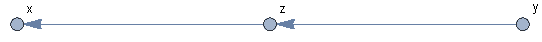
\includegraphics[scale=0.8, center]{images/equivalent_graph.pdf}   
\end{example}

\begin{exercise}
Show that the graph
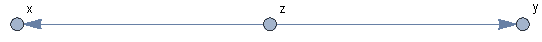
\includegraphics[scale=0.8, left]{images/graph_exercise.pdf}
 also implies the independence of $x$ and $y$ given $z$.
\end{exercise}

\begin{example}[Conditional Independence Test]
We want to implement a function \texttt{IsConditionalIndependent}, which returns \texttt{True} if \texttt{sourceNode} is conditionally independent of \texttt{targetNode} given a list of \texttt{conditionalNodes} for \texttt{graph}, otherwise \texttt{False}.\\

The implemented algorithm works as follows:\\
\begin{itemize}
\item
If \texttt{sourceNode} and \texttt{targetNode} are identical, then they are dependent.
\item
If there exist undirected paths between \texttt{sourceNode} and \texttt{targetNode} and one of these paths has only two nodes, \texttt{sourceNode} and \texttt{targetNode} are directly connected and dependent.
\item
If there is no undirected path between \texttt{sourceNode} and \texttt{targetNode}, they are independent.
\item
If all paths contain at least one segment with 3 nodes, which is not a v-structure and the center node is in \texttt{conditionalNodes}, \texttt{sourceNode} and \texttt{targetNode} are independent.
\item
If all paths contain at least one segment with 3 nodes, which is a v-structure and the center node and all its descendants are not in \texttt{conditionalNodes}, \texttt{sourceNode} and \texttt{targetNode} are independent, else they are dependent. 
\end{itemize}

\begin{mathematica}
IsConditionalIndependent[g_Graph,
                         sourceNode_Integer,
                         targetNode_Integer,
                         conditionalNodes_List]:= Module[
    {paths, blockedPathSegments},
    (* source and target node are identical *)
    If[sourceNode == targetNode,
       Return[False]];
    paths = FindPath[UndirectedGraph[g], sourceNode, targetNode,
                     Infinity, All];
    (* there is a direct path between source and target node *)
    If[AnyTrue[paths, Length[#] == 2 &],
       Return[False]];
    (* there is no path between source and target node *)
    If[Length[paths] == 0,
       Return[True]];
    (* partition each path into overlapping segments of 3 nodes *)
    paths = Map[Partition[#, 3, 1] &,
                paths];
    (* get all paths, which are not blocked by a a conditional node *)
    blockedPathSegments = Map[Not[EdgeQ[g, #[[1]] \[DirectedEdge] #[[2]]] && 
                                  EdgeQ[g, #[[3]] \[DirectedEdge] #[[2]]]] && 
                                  MemberQ[conditionalNodes, #[[2]]]  &,
                              paths, {2}];
    paths = Pick[paths, Map[Not[AnyTrue[#, TrueQ]] &, blockedPathSegments]];
    If[Length[paths] == 0,
       Return[True]];
    (* get all paths, which are not blocked by a v-structure *)
    blockedPathSegments = Map[EdgeQ[g, #[[1]] \[DirectedEdge] #[[2]]] && 
                              EdgeQ[g, #[[3]] \[DirectedEdge] #[[2]]] && 
                              Not[MemberQ[conditionalNodes, #[[2]]]] &&
                              Length[Intersection[VertexOutComponent[g, #[[2]]],
                                                  conditionalNodes]] == 0  &,
                              paths, {2}];
    paths = Pick[paths, Map[Not[AnyTrue[#, TrueQ]] &, blockedPathSegments]];
    If[Length[paths] == 0,
       Return[True],
       Return[False]];
    ]

g = Graph[{1 \[DirectedEdge] 3, 2 \[DirectedEdge] 3, 3 \[DirectedEdge] 4},
          VertexLabels -> {1 -> "x", 2 -> "y", 3 -> "z", 4 -> "w"}];
IsConditionalIndependent[g, 1, 2, {4}]       
\end{mathematica}
returns \texttt{False} for the graph\\

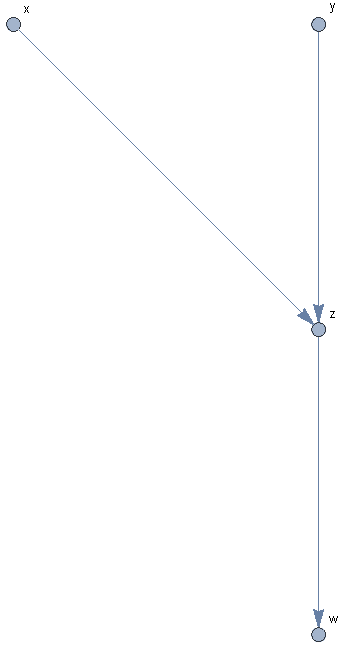
\includegraphics[scale=0.8, center]{images/v_structure_with_descendant.pdf}

which states that $x$ is not independent of $y$ given $w$ even if $x$, $y$ and $z$ are nodes of a v-structure.\\

To verify this statement, we write down the joint distribution for this graph
\begin{equation}
p(x,y,z,w)=p(w\,\vert\, z)p(z\,\vert\, x,y)p(x)p(y)
\end{equation}
We marginalize over $z$ and condition on $w$.
\begin{equation}
p(x,y\,\vert\,w)=\int_{-\infty}^{+\infty}dz \frac{p(x,y,z,w)}{p(w)}=p(x)p(y)\int_{-\infty}^{+\infty}dz \frac{p(w\,\vert\, z)p(z\,\vert\, x,y)}{p(w)}
\end{equation}
which does not factor into a product of $x$ and $y$. For some special probability densities it could happen that the factorization occurs, but in general $x$ and $y$ are dependent, which agrees with the result of the function \texttt{IsConditionalIndependent}. The independence relation is broken in the case of a v-structure if any descendants of the center node is conditioned on.
\end{example}
\begin{exercise}
Apply the function \texttt{IsConditionalIndependent} to the graph

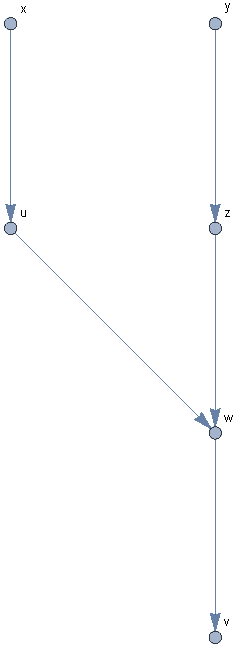
\includegraphics[scale=0.8, center]{images/complex_graph.pdf}

and check under which conditions node $x$ and $y$ are independent when conditioned on a certain subset of the remaining nodes.
\end{exercise}

\section{Time Series}
We now want to apply graphical models to the analysis of time series data \cite{barber2010}. A time series can be represented by a sequence of random variables $x_{1:T}$, which are associated with a sequence of time points $t_{1:T}$. A time point can be e.g. 01 Jan 1970 00:00:00.000, which has a resolution of milliseconds, but depending on your application a higher resolution may be necessary such as nanoseconds and therefore more digits after decimal point. We also use the notation $x_t$, where $t$ stands for the index associated with current time $t$, and $x_{t-1}$ means the random variable at the previous time point and $x_{t+1}$ the random variable at the next future time point and so on.\\

The Wolfram Language has the built-in symbol \texttt{TimeSeries} as a wrapper around a list of time-value pairs $\{t_{i},x_{i}\}$, where $x_{i}$ can be a scalar or an array and $t_{i}$ can be numeric or \texttt{AbsoluteTime} e.g. \texttt{AbsoluteTime["01 Jan 1900 00:00:00.000"]}, which returns the result \texttt{0} as the number of seconds since the beginning of January 1, 1900 in your local timezone. Local time has typically an offset to GMT in multiple of hours including daylight savings, which is given by \texttt{\$TimeZone}. Therefore the number of seconds returned by \texttt{AbsoluteTime} is the same on each computer in the world, where the code is executed.

\begin{remark}
If you specify a timezone explictly e.g.\\

\texttt{AbsoluteTime["01 Jan 1900 00:00:00.000", TimeZone -> 0]},\\

the returned number is non-zero and a multiple of 3600, because it calculates the difference between January 1, 1900 00:00:00 GMT and January 1, 1900 00:00:00 in your local timezone.
\end{remark}

\begin{remark}
\texttt{AbsoluteTime} does not take into account leap seconds. Therefore the difference between two calendar dates calculated by \texttt{AbsoluteTime} will differ by the amount of leap seconds, which were introduced in this time interval.   
\end{remark}

We want to study a probabilistic model based on the following subgraph\\
     
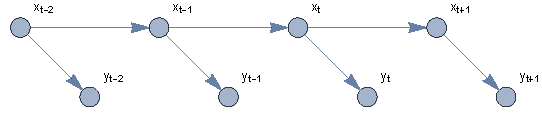
\includegraphics[scale=1.2, center]{images/time_series_graph.pdf}

The idea behind this model is that the system is fully described by the variable $x$ and there are observations $y$, which determine $x$ completely or partially depending on the measurement process. The system state $x$ is not directly observable, nevertheless we want to predict the future system state based on all its observations and some prior knowledge of $x$.\\

The system state $x$ also fulfills the Markov property.

\begin{definition}[Markov Property]
  \label{th:markovproperty}
  \index{markov property}
  The system state $x_t$ is completely determined by the previous state $x_{t-1}$ only, which can be written as
\begin{equation}
p(x_t\,\vert\, x_{t-1},x_{t-2},\ldots,x_{t-n})=p(x_t\,\vert\, x_{t-1})
\end{equation}
\end{definition} 
The property can be directly read off the graph, because if we condition on $x_{t-1}$, $x_t$ become conditionally independent of its complete past history $x_{t-2},\ldots$ as we have shown in example \ref{ex:chain_graph}.

\begin{exercise}
A graph like

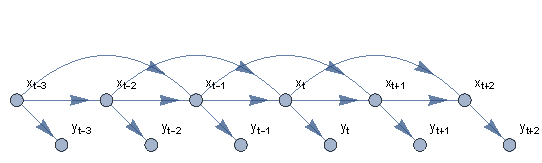
\includegraphics[scale=1.2, center]{images/non_markov_graph.pdf}

does not fulfill the Markov property. Show that by merging two $x$ nodes and two $y$ nodes to new nodes $z$ and $o$, the new graph takes the form

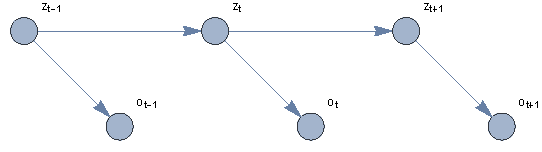
\includegraphics[scale=1.0, center]{images/markov_graph.pdf}

with $z_{t-1}=\{x_{t-3},x_{t-2}\}$, $o_{t-1}=\{y_{t-3},y_{t-2}\}$, $z_t=\{x_{t-1},x_t\}$, $o_t=\{y_{t-1},y_t\}$, $z_{t+1}=\{x_{t+1},x_{t+2}\}$, $o_{t+1}=\{y_{t+1},y_{t+2}\}$ and fulfills the Markov property.  
\end{exercise}


The joint probability density can be immediately written down as a recursive equation
\begin{equation}
p(x_{t+1},y_{t+1},x_{t},y_{t},\ldots)=p(x_{t+1}\,\vert\, x_{t})p(y_{t+1}\,\vert\, x_{t+1})p(x_{t},y_{t},x_{t-1},y_{t-1},\ldots)
\end{equation}
We are only interested to predict $x_{t+1}$, so we marginalize over all previous system states $x_{t},x_{t-1},\ldots$.

\begin{equation}
\begin{aligned}
p(x_{t+1},y_{t+1},y_{t},\ldots)&=\int_{-\infty}^{+\infty}dx_{t}\int_{-\infty}^{+\infty}dx_{t-1}\ldots p(x_{t+1},y_{t+1},x_{t},y_{t},\ldots)\\
&=p(y_{t+1}\,\vert\, x_{t+1})\int_{-\infty}^{+\infty}dx_{t} p(x_{t+1}\,\vert\, x_{t})\int_{-\infty}^{+\infty}dx_{t-1}\ldots p(x_{t},y_{t},x_{t-1},y_{t-1},\ldots)\\
&=p(y_{t+1}\,\vert\, x_{t+1})\int_{-\infty}^{+\infty}dx_{t} p(x_{t+1}\,\vert\, x_{t}) p(x_{t},y_{t},y_{t-1},\ldots)
\end{aligned}
\end{equation}
We now condition on all the observations $y_{t+1},y_{t},\ldots$
\begin{equation}
\begin{aligned}
p(x_{t+1}\,\vert\, y_{t+1},y_{t},\ldots)&=\frac{p(x_{t+1},y_{t+1},y_{t},\ldots)}{p(y_{t+1},y_{t},\ldots)}
=\frac{p(x_{t+1},y_{t+1},y_{t},\ldots)}{p(y_{t+1}\,\vert\, y_{t},\ldots)p(y_{t},\ldots)}\\
&=\frac{1}{p(y_{t+1}\,\vert\, y_{t},\ldots)}p(y_{t+1}\,\vert\, x_{t+1})\int_{-\infty}^{+\infty}dx_{t} p(x_{t+1}\,\vert\, x_{t}) \underbrace{\frac{p(x_{t},y_{t},y_{t-1},\ldots)}{p(y_{t},\ldots)}}_{p(x_{t}\,\vert\,\ y_{t},y_{t-1},\ldots)}
\end{aligned}
\end{equation}
This recursive equation is the mathematical fundament of the Bayes filter \cite{gustafsson2012}.\\

\begin{definition}[Bayes Filter]
  \label{th:bayesfilter}
  \index{bayes filter}
  The probability density $p(x_{t+1}\,\vert\, y_{t+1},y_{t},\ldots)$ can be calculated iteratively from the last known $p(x_{t}\,\vert\,\ y_{t},y_{t-1},\ldots)$ by a prediction step 
\begin{equation}
p(x_{t+1}\,\vert\, y_{t},\ldots)=\int_{-\infty}^{+\infty}dx_{t} p(x_{t+1}\,\vert\, x_{t}) p(x_{t}\,\vert\, y_{t},y_{t-1},\ldots)
\end{equation}
followed by a correction step
\begin{equation}
p(x_{t+1}\,\vert\, y_{t+1},y_{t},\ldots)=\frac{p(y_{t+1}\,\vert\, x_{t+1})}{p(y_{t+1}\,\vert\, y_{t},\ldots)}p(x_{t+1}\,\vert\, y_{t},\ldots)
\end{equation}
$p(x_{t+1}\,\vert\, x_{t})$ describes the time evolution of the system and $p(y_{t+1}\,\vert\, x_{t+1})$ the measurement process of the system state. If the system state is controlled by an external input $u_t$, it is only necessary to modify $p(x_{t+1}\,\vert\, x_{t})$ by $p(x_{t+1}\,\vert\, x_{t}, u_{t})$. 
\end{definition}

The Bayes filter estimates the state at time $t+1$ from the all the previous states and observations, but how do we start the iteration or what can we say about the system state without any observations?\\

It turns out that the prior state estimate $p(x_0)$ before any observations are made can be chosen as a constant. After the first correction step when the normalization is performed the constant will anyhow be cancelled out and the state estimate will improve with each update.\\  

The Bayes filter framework is the conceptual basis of a large number of existing models like Kalman and Particle filters (which will be covered in the next sections of this chapter), Hidden Markov Models (see next example), Dynamic Bayesian Networks (basically the introduction in this chapter) and Markov Decision Processes (which will be covered in the context of reinforcement learning in the next chapter) with a wide range of applications.

\begin{example}[Graph World]
We want to study a simple system called Graph World, which is a generalization of the Grid World system often used as an introductory example in reinforcement learning.\\

The system consists of a finite number of states $1,2,\ldots,k$ and a $k\times k$ transition matrix $P_{ij}$, which describes the probabilities of a transition from state $i$ to state $j$. $P_{ij}$ is also an adjacency matrix with an associated graph structure, where the vertices are the system states and the directed edges with an assigned weight corresponding to the probability that a transition from a source to a target node happens (a probability $0$ means that such a transition never happens and therefore no edge is drawn in this case).\\

% We further introduce a measurement process, which is based on an observer node % $o$, which measures the number of edges in the shortest path from node $o$ to the % current system state node $i$. The shortest path computation ignores the weight % and direction of each edge.\\

We further introduce a measurement process, which returns with a probability $p$ the right state $i$ the system is currently in and with probability $1-p$ a wrong state $j \neq i$. So the pure measurement would give us the right prediction only with probability $p$. Let's see if the application of the Bayes filter can improve the prediction accuracy.\\

Let's assume that the system is in state $i$ at $t_0$ and in the next time step $t_1$, it will transition to another state $j$, where $P_{ij}\neq 0$. It is also possible that the system remains in the same state at $t_1$ if $P_{ii}\neq 0$. At the beginning the first state is unknown and we start with a prior state estimate of $p(x_0)=\frac{1}{k}\sum_{i=1}^{k}\delta(x-i)$.\\

We write first a function \texttt{GraphWorld}, which constructs a random graph world from a list of node names, which provide a textual label for each node, and the length of history of states. It returns key-value pairs with 3 pre-defined keys: a key \texttt{"graph"} with an associated \texttt{Graph} object, a key \texttt{"transition\_probabilities"} with the matrix $P_{ij}$, a key \texttt{history} with a sequence of states, which are generated from a random initial state, and a graphical representation of the state history with key \texttt{"timeline"}.

\begin{mathematica}
GraphWorld[nodeLabels_List, historyLength_Integer] := Module[
   {graph, transitionMatrix, history, world, numNodes, labels, 
   initialState, nodes, dists, edges, historyGraph},
   numNodes = Length[nodeLabels];
   nodes = Range[numNodes];
   labels = MapThread[#1 -> #2 &, {nodes, nodeLabels}];
   transitionMatrix = RandomChoice[{0, 1}, {numNodes, numNodes}];
   (* There could be a row with only zeros, where no transitions to
      another node occurs. To avoid this situation, a random unit
      vector will replace such a row.
    *)
   transitionMatrix = Map[If[Total[#] == 0, 
                          UnitVector[Length[#], RandomChoice[nodes]], #] &, 
                          transitionMatrix];
   (* A graphical representation of all possible state transitions, which can occur
      in this world.
    *)
   graph = AdjacencyGraph[transitionMatrix, VertexLabels -> labels];
   (* Normalize each row of the transition matrix *)
   transitionMatrix = Map[#/Total[#] &, transitionMatrix];
   initialState = RandomChoice[nodes];
   (* Create an empirical distribution for each node from the transition matrix *)
   dists = Map[EmpiricalDistribution[# -> nodes] &,
               transitionMatrix];
   (* Starting with a random initial state, sample a new state from the old state
      using the empirical distributions and collect them in a list.
    *)
   history = NestList[RandomVariate[dists[[#]]] &,
                      initialState, historyLength];
   (* Create a graphical representation of the state transitions as directed graph,
      where each edge represents a time step from node at time t to the node at time
      t + 1.
    *)
   edges = Partition[history, 2, 1];
   historyGraph = Graph[Table[Labeled[i \[DirectedEdge] i + 1, i],
                              {i, 1, Length[edges]}],
    VertexLabels -> Append[Table[i -> nodeLabels[[edges[[i, 1]]]],
                                 {i, 1, Length[edges]}],
                    Length[edges] + 1 -> nodeLabels[[edges[[Length[edges], 2]]]]]];
   world = Association["graph" -> graph, 
                       "transition_probabilities" -> Transpose[transitionMatrix],
                       "history" -> history ,
                       "timeline" -> historyGraph];
   Return[world]]

SeedRandom[123456789];   
world = GraphWorld[Characters["abcdefg"], 10];
world["graph"]
\end{mathematica}

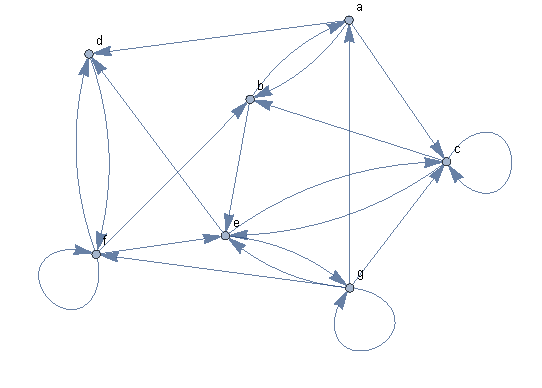
\includegraphics[scale=0.9, center]{images/graph_world.pdf}

\begin{mathematica}
world["timeline"]
\end{mathematica}
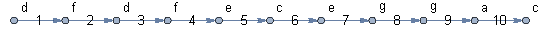
\includegraphics[scale=1.2, center]{images/state_history.pdf}

The timeline graph shows the sequence of states at $t_0,t_1,\ldots$ and the edge $i$ represents a transition from state at $t_{i-1}$ to the state at $t_{i}$. We assume that there are no measurements before $t_1$.\\ 

In the next step we implement a measurement function \texttt{MeasurementProcess}, which gets a world as the first argument, on which the measurement is performed, and an observer node \texttt{observerNode} and returns a list of distributions for each time step of the world history. Each distribution has as many elements as number of nodes in the graph and the values represent the probability that the graph distance of a node to the observer node is compatible with the distance measurement of the system state. If the graph distance would unambiguously determine the system state, only one element would be $1$ and the others would be $0$, but there are typically more nodes with the same graph distance. Because the measurement cannot distinguish between these nodes, they have equal probability to be the actual system state.\\

Wolfram Language provides the function \texttt{GraphDistance}, which returns the number edges of the shortest path between two nodes in a graph. If two nodes are not connected, the graph distance will be \texttt{Infinity}.    

\begin{mathematica}
MeasurementProcess[world_, observerNode_] := Module[
   {measurements, distances, size, distributions},
   (* Calculate a list of measurements of the graph distance between the
      observer node and all the system states in the world's history
      excluding the initial system state.
    *)
   measurements = Map[GraphDistance[world["graph"], observerNode, #]&,
                      world["history"][[2 ;; All]]];
   (* Calculate the graph distances between the observer node and all other
      graph nodes. *)
   distances = GraphDistance[world["graph"], observerNode];
   size = Length[distances];
   (* Calculate the measurement distribution for each time step by checking,
      which node has the same graph distance than the measurement. 
    *)
   distributions = Boole[Map[MapThread[Equal, {distances, Table[#, size]}] &,
                             measurements]];
   (* Normalize each row so that the values can be interpreted as
      probabilities. *)
   distributions = Map[# / Total[#]&, distributions]; 
   Return[distributions]]
   
measurements = MeasurementProcess[world, 2];
\end{mathematica}

The observer node is chosen to be b.\\

The Bayes filtering starts with an initial distribution of states reflecting our prior knowledge about the system state at $t_0$. Because we have no prior knowledge at this point, we choose a uniform distribution over all possible states or nodes of the graph.

\begin{mathematica}
nodes = Characters["abcdefg"];
stateDistribution = AssociationThread[nodes -> Table[1/Length[nodes],
                                                     Length[nodes]]];
\end{mathematica}

Then we apply the transition matrix to this distribution in the prediction step.

\begin{mathematica}
stateDistribution = AssociationThread[nodes -> world["transition_probabilities"].
                                      Values[stateDistribution]];
\end{mathematica}

In the correction step we multiply with the first element of the distributions returned by \texttt{MeasurementProcess} and normalize the result.  

\begin{mathematica}
stateDistribution = AssociationThread[nodes -> measurements[[1]] *
                                      Values[stateDistribution]];
stateDistribution = If[Total[stateDistribution] == 0,
                       AssociationThread[nodes -> Table[1/Length[nodes],
                                                        Length[nodes]]],
                       stateDistribution / Total[stateDistribution]];
\end{mathematica}

This gives the estimated state distribution at time step $t_1$.

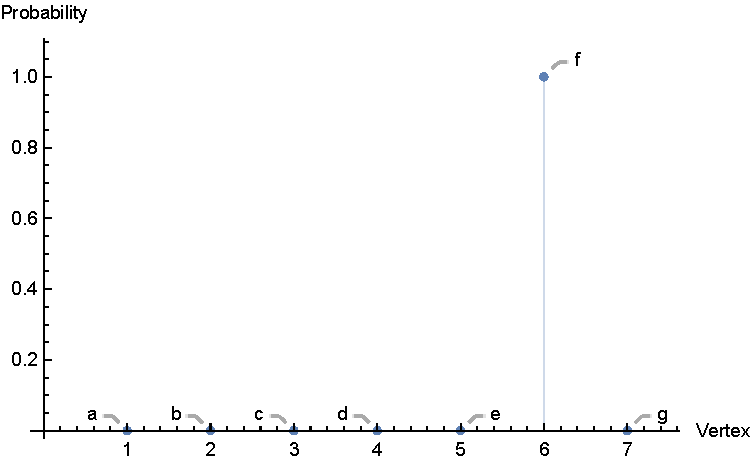
\includegraphics[scale=0.8, center]{images/state_estimate_t1.pdf}

We repeat the steps for $t_2$ with the result

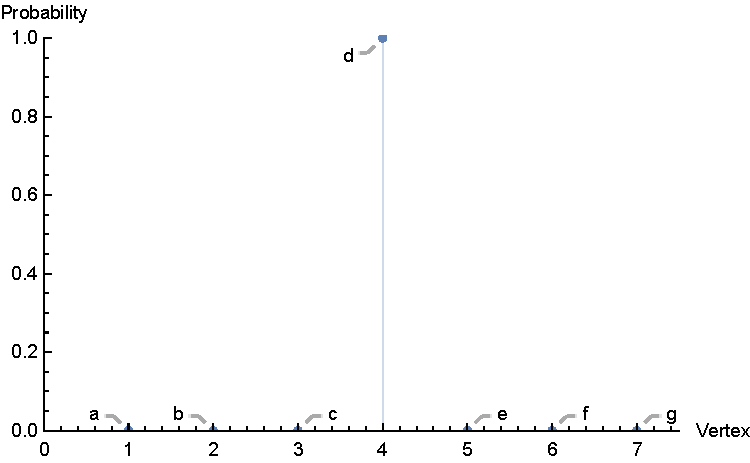
\includegraphics[scale=0.8, center]{images/state_estimate_t2.pdf}

and for $t_3$

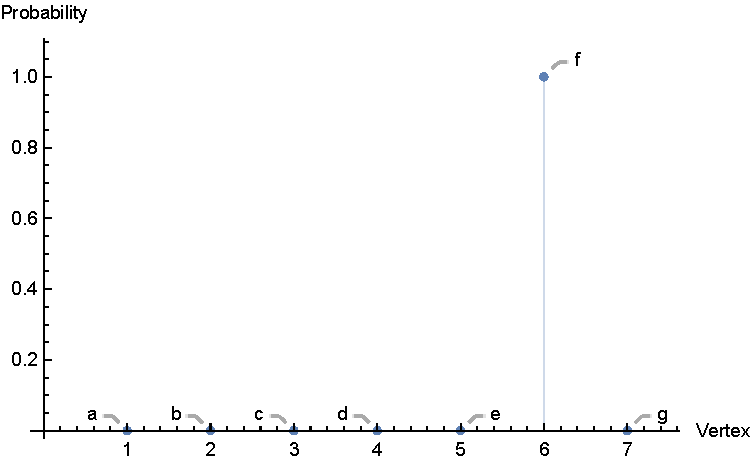
\includegraphics[scale=0.8, center]{images/state_estimate_t3.pdf}

If we take the state with the maximum probability, the state estimates at $t_1$, $t_2$ and $t_3$ are f, d and f, which agrees perfectly with the timeline graph.\\

Also at $t_4$ the system state is correctly predicted as e, but at $t_5$ the states c, d and g have all the same probability and the correct state cannot be unambiguously estimated.

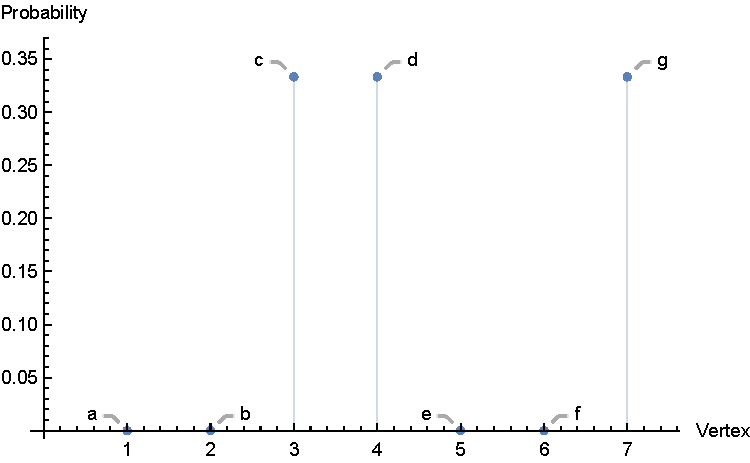
\includegraphics[scale=0.8, center]{images/state_estimate_t5.pdf}

The reason for this ambiguity is shown in the next figure, where the red edges mark all transitions from the previous state e at $t_4$ to the possible next states at $t_5$. The blue edges highlight the shortest paths from the observer node b to these states and they all have the same graph distance $2$.

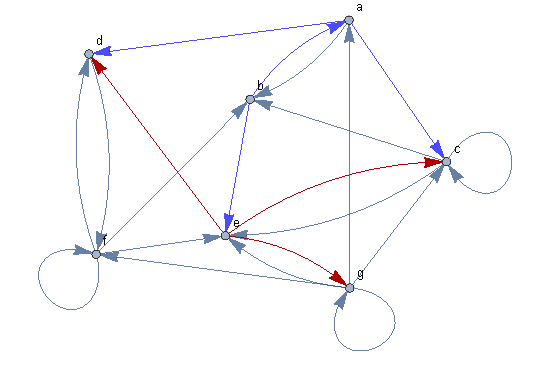
\includegraphics[scale=0.8, center]{images/highlighted_graph_world.pdf}

Therefore it is not possible to identify the correct state at $t_5$ based on this measurement.   

\end{example}

\begin{exercise}
Modify the parameter of the last example e.g. the observer node or the number of nodes in the graph to get an deeper understanding how the Bayes filter works.
\end{exercise}

\section{Kalman Filter}

\section{Particle Filter}

\chapter{Probabilistic Models (Applications)}

\begin{summary}
  This chapter covers the whole range of probabilistic models from simple to complex ones. We show that the simple models can be used as building blocks for simulating real-world systems.
\end{summary}

\section{Poisson Clock}
A very simplified model of a clock is the Poisson clock, where the tick counts $x$ are Poisson-distributed.

\begin{definition}[Poisson Clock]
  \label{th:poissonclock}
  \index{poisson clock}
  \begin{equation}
    \mathcal{P}(x\,\vert\, \lambda\rightarrow\nu t)=\sum_{k=0}^{\infty}\frac{\nu^k t^k}{k!}\exp(-\nu t)\delta(x-k)
  \end{equation}
  $\nu$ is the clock rate (number of ticks in a certain time interval) and $t$ is the elapsed time. Because the expectation value is $\mu=\lambda t$, the tick count is a measure of time.
\end{definition}
However, this is not a good model of a real clock, because there is only one parameter $\nu$, which controls the clock rate, and the clock noise is completely determined by this choice. In a real clock model you can control the rate and the noise independently.

Nevertheless, the Poisson clock is used very often for e.g. simulating the arrival of costumers in a shop or the number of decays of a radioactive material. It is also a building block of the Ptolemy II simulation framework \cite{ptolemy2003}. 
\section{Gaussian Lattice Model}
The Gaussian Lattice Model is a variant of the famous Ising Model \cite{mussardo2010}. We want to study this model in the one-dimensional case, where it can be solved exactly.

\section{Random Matrices}
A random matrix $m$ is $N\times N$ matrix with its elements $m_{ij}\sim p(x)$ \cite{livan2017}.

%---------------------------------------------------------------------------
% Bibliography
%---------------------------------------------------------------------------

\addcontentsline{toc}{chapter}{\textcolor{tssteelblue}{Literature}}
\printbibliography{}

%---------------------------------------------------------------------------
% Index
%---------------------------------------------------------------------------

\printindex

\end{document}
